\documentclass[a4paper,12pt]{book}


  % a file containing your definitions, which packages to load etc
    \usepackage{amssymb}
  \usepackage{latexsym}
  \usepackage{amsfonts}
  \usepackage{amsthm}
  \usepackage{amsmath}


% put your command and environment definitions here

 \newcommand{\needscitation}[2]{\textcolor{red}{\textbf{#1} (from: #2)}}

 \newcommand{\red}[1]{\textcolor{red}{#1}}
 \newcommand{\TODO}{\textcolor{red}{TODO}}
 \newcommand{\todo}{\textcolor{red}{TODO}}



% Some theorem environments
% remove "[theorem]" if you do not want them to use the same number sequence


  \newtheorem{theorem}{Theorem}[chapter]
  \newtheorem{lemma}[theorem]{Lemma}
  \newtheorem{proposition}[theorem]{Proposition}
  \newtheorem{corollary}[theorem]{Corollary}

  \newtheorem{conj}{Conjecture}
  \renewcommand{\theconj}{\Alph{conj}}  % numbered A, B, C etc

  \theoremstyle{definition}
  \newtheorem{definition}[theorem]{Definition}
  \newtheorem{example}[theorem]{Example}
  \newtheorem{examples}[theorem]{Examples}
  \newtheorem{question}[theorem]{Question}
  \newtheorem{remark}[theorem]{Remark}
  \newtheorem{notn}[theorem]{Notation}

  


  % line-spacing factor
  \renewcommand{\baselinestretch}{1.2}

  % use this if you don't want headers and page numbers on
  % blank pages at the end of chapters
  \newcommand{\blanknonumber}{\newpage\thispagestyle{empty}}

  % needed for ANU logo on titlepage (optional)
  \usepackage{graphicx}
  \usepackage{physics}
  \usepackage{alias}
  \usepackage{mathtools}
  \usepackage{algorithm}
  \usepackage{algpseudocodex}

  % margins
  \setlength{\voffset}{-1in}
  \setlength{\hoffset}{-1in}
  \setlength{\oddsidemargin}{4cm}
  \setlength{\evensidemargin}{2.5cm}
  \setlength{\textwidth}{14.5cm}
  \setlength{\textheight}{22.5cm}
  \setlength{\topmargin}{2.5cm}


\usepackage{url}
\usepackage[hidelinks]{hyperref} %added by Joan Licata,  2022
\usepackage{xcolor}
  % for working drafts, un-comment the following command and list
  % the chapters etc you want to see in the output, eg
  % \includeonly{titlepage,chapter1,chapter2}



\begin{document}


  % set page numbers to roman and suppress chapter numbers
  \frontmatter

  % remove or switch the order of these as you see fit
  \begin{titlepage}
\begin{center}

\vspace*{\fill} \Huge
                        Simulations in AC Tokamak Ramp Downs
\\
\vfill\vfill\Large
                          Thomas Malcolm
\\
\vfill\vfill
                          Sep 2023
\\
\vfill\vfill \normalsize
         A thesis submitted for the degree of \\
         \emph{Bachelor of Mathematical Sciences (Honours)} \\
         of the Australian National University
\vfill
         
\includegraphics{ANU.eps}

\end{center}

\end{titlepage}
\blanknonumber

  

\blanknonumber\ \blanknonumber

\vspace*{\fill}

\begin{center}\emph{
%
For George, Paul, Ringo and John.
%
}
\end{center}

\vfill\vfill\vfill
\blanknonumber
  
  
\chapter*{Declaration}\label{declaration}
\thispagestyle{empty}
The work in this thesis is my own except where otherwise stated.

\vspace{1in}


\hfill\hfill\hfill
%
Thomas Malcolm.
%
\hspace*{\fill}
\blanknonumber
  
  
\chapter*{Acknowledgements}\label{acknowledgements}
\addcontentsline{toc}{chapter}{Acknowledgements}


First and foremost I'd like to thank Matthew Hole, my supervisor. I came 
into this year a little daunted at the prospect of tackling a physics-based 
project with a physics background not extending past ``A Brief History of Time''.
Your patience and willingness to explain concepts to me I'll forever appreciate, 
and your energetic approach to problem solving made me feel both at home and excited 
for the work we have done in this thesis. Thank you for always taking the time to talk to 
me, and for being a fantastic supervisor.

In a similar vein, thank you to the rest of the Plasma Theory and Modelling group for always being 
willing to answers questions when I had them. You guys were definitely my saving grace 
at times, and I only wish I spent more time getting to know you all this year. I should give 
a special shout out to Nick, Sandra, Dean and Josh specifically for being so 
accommodating, helpful, and kind in answering my questions when I would pop around. 

I'd like to thank the other Honours students for helping make this a fantastic 
year. Our little nook of MSI proved very distracting, but in the best possible 
way. Also Joe gets a special shout out purely to spite everyone else.

Last but certainly not least, to Kirsten and Graeme. Thank you for your support these last 
couple years we've known each other, and the infinite kindness you give to all those around you. However silly it is,
your encouragement genuinely helped motivate me at times, and it was always my pleasure having the 
opportunity to rant to you about whatever problem I was working on at the time, and how insurmountable
it seemed! Yet each time you had confidence it would all work out fine, and then somehow it always would. I can only assume 
this is some wizardry I am not yet privy to, but am nevertheless indebted to your kindness and hospitality.\blanknonumber
  
  \chapter*{Abstract}\label{abstract}

\addcontentsline{toc}{chapter}{Abstract}



% your abstract goes here
\blanknonumber
  
  \tableofcontents\blanknonumber
  
  

\chapter{Notation and terminology}\label{notation}
%\addcontentsline{toc}{chapter}{Notation and terminology}

\renewcommand{\thefootnote}{\fnsymbol{footnote}}


\

\noindent\textbf{Notation}

% adjust the lengths to suit your needs (difference of .22cm works best)

\newcommand{\nttn}[2]{\item[{\ \makebox[3.18cm][l]{#1}}]{#2}}
\begin{list}{}{ \setlength{\leftmargin}{3.4cm}
                \setlength{\labelwidth}{3.4cm}}

\nttn{$L^2(\R^n)$}{Space of $L^2$ integrable functions on $\R^n$}

\nttn{$B_0$}{On-axis magnetic field}
\nttn{$R_0$}{Major radius (Tokamak)}
\nttn{$a$}{Minor radius (Tokamak)}
\nttn{$\Psi$}{Poloidal magnetic flux function}
\nttn{$j_{\phi}$}{Toroidal current density}
\nttn{$J_{\phi}$}{Normalised toroidal current density (normalised w.r.t. $B_0$)}
\nttn{$p$}{Plasma pressure density}

\end{list}

\

\noindent\textbf{Terminology}

% adjust the lengths to suit your needs (difference of .22cm works best)

\newcommand{\term}[2]{\item[{\ \makebox[4.58cm][l]{#1}}]{#2}}
\begin{list}{}{ \setlength{\leftmargin}{4.8cm}
                \setlength{\labelwidth}{4.8cm}}


\term{GS / GSE}{Grad-Shafranov equation}
\term{GSH}{Grad-Shafranov-Helmholtz equation}
\term{MHD}{Magnetohydrodynamics}


\end{list}
\blanknonumber

  % \include{background}\blanknonumber

  % set page numbers to arabic, reset to 1
  \mainmatter

  % Chapters of thesis
  
\chapter{Introduction}
\label{chapter1}

% 1.1.
\section{Plasma Science}

This thesis is multidisciplenary by nature, incorporating aspects of mathematics, physics and computer science throughout 
the various challenges faced in reaching the conclusions we have. 


Before burying ourselves in the thick of our results we 
will cover the requisite knowledge for working in the plasma science simulation space. First we'll discuss what 
the physical object of our attention (``plasma'') actually is, with a brief discussion on the design of fusion reactors, where we will 
emphasise the structures that specifically relate to our interests. In the background chapter we will expound on this by 
building the mathematical theory underpinning physical processes within the fusion reactor, providing us a way to reason
about the behaviour of plasma (and related processes) inside a fusion reactor, or, more accurately, approximate their behaviour 
via simulation.




% 1.1.1.
\subsection{I'm a Mathematician... what is ``plasma''?}

While an initially daunting topic, fear not fearful mathematician, for many of the inherently physical 
behaviours in plasma science we require can be expressed in terms of our dearest mathematical expressions -- differential equations! 
But first, what actually is ``plasma''? Webster's dictionary defines plasma to be ``a green faintly translucent quartz'' \cite{websters_plasma}. 
While I'm sure there isn't no relation between crystals and our investigations, this is unfortunately, not the recipient of our affection. 

When plasma is referred to in everyday conversation it is often noted as being the ``4th state of matter''. To introduce slightly more rigour,
plasma is an extension of the gaseous state of matter, where its energy (read: temperature) is increased sufficiently high that the electrons 
are no longer bound by the electromagnetic force to the atom's nucleus \cite{basics-of-plasma-astrophysics}. The resulting substance is a ``pool'' of cations (the positively charged nuclei), and 
electrons (negatively charged), that exhibits interesting properties. It is these properties that we seek to exploit in the search of controlled, 
sustained fusion reactions.

Plasma is abundant in nature -- just not in many places that we as Humans commonly look. Stars are the most immediate example of matter in a plasma state, 
and are readily viewable (at least for half the day). Lightning strikes are paths through the atmosphere which are ionised, 
and neon signs work by heating Neon gas within a tube to ionise it \cite{plasma-lightning}.

The question then is, what is ``fusion'', and how does this relate to plasma? The answer comes back to energy. Analogously to a fission reaction, 
where energy is released through the division of atoms, one can also fuse two separate atoms together and have large amounts of energy emitted 
as a bi-product of that fusion. It is (essentially) this extra energy that we wish to harness when harvesting energy from a fusion reactor.

While there are no shortages of elements that can theoretically be used to fuel a fusion reactor, the one most commonly associated with fusion is Deuterium -- a stable isotope of Hydrogen that 
has a neutron in its nucleus (whereas a 'standard' Hydrogen atom contains only a single proton). Analogously, Tritium is an isotope of Hydrogen
that has two neutrons in its nucleus (though is much less stable). Consider the fusion of a Deuterium atom with a Tritium atom:
\[ \prescript{2}{}{\text{H}} + \prescript{3}{}{\text{H}} \stackrel{\text{(fusion)}}{\to} \prescript{4}{}{\text{He}} + n + 17.59 \, \text{MeV} \]

Here two Hydrogen isotopes fuse together to form a single Helium-$4$ atom, and in the process of doing so release 
a single neutron and $17.59$ MeV of energy. This excess energy is what is so attractive about fusion processes as a sustainable 
energy source -- for such little input we receive a substantial amount of energy, and at that, using one of the most abundant 
resources available on Earth; water.

The question then becomes, how do we drive this fusion process? If two atoms can fuse as such, why do we not 
see atoms fusing everywhere around us accompanied by violent explosions destroying all that we've 
come to know and love? The answer is that we kind of do -- just not normally in the places that humans expect to be inhabiting. In fact, we see this happening everyday --
for those of us fortunate enough to be able to see the sun that is. Our sun 
is a large ball of plasma where an estimated $9.3 \times 10^{37}$ fusion reactions are expected to occur every second \cite{nasa-sun-fusion}, 
and is one of the easiest examples of both plasma as a state of matter, and of a self-sustaining fusion reaction.

How then do two hydrogen atoms fuse -- how can we create a sun on Earth? The nucleus of an atom (consisting of positively charged 
protons, and neutral neutrons) is positively charged, and so two atoms' nuclei will repel each other due to the Coulomb force when pushed together. This is the force 
we have to overcome to enable a fusion reaction to take place (and what stops the world around us burning!). To overcome this the process is relatively ``simple'' -- 
we just increase the energy of our atoms so that when they collide they collide with enough energy to overcome this force, allowing the strong force to become
dominant, fusing the two atoms. When we energise a mass (take a gas here) of atoms enough, they become ionised however, which is 
exactly the state of plasma we described earlier. In other words, if we want to reason about the creation, sustainment, and effects of 
fusion reactions, we need first to understand the dynamics of plasma, the medium in which the fusion reactions take place. From this comes a plethora of questions, ranging from 
``how do we generate such a plasma?'' to ``how do we reliably control such a plasma'' and ``how do we harness such a plasma''? Alas, we 
digress however, as we do not seek to solve the big problems in fusion science in this here mere mortal thesis. Instead, now equipped 
with at least a passing knowledge of what constitutes a ``plasma'' state and what it means for a fusion reaction to take place, 
we will humbly delve into the inner workings of fusion reactor terminology and design.


% 1.1.2.
\subsection{Fusion Reactor Design 101}

Here we will discuss the important structural aspects of a Tokamak fusion reactor. The term ``Tokamak'' is a 
Russian acronym which translates as ``toroidal chamber with magnetic coils'' \cite{iter-tokamak-acronym}. Aptly, a Tokamak is a toroidal 
object which is used as a vessell for plasma which is driven via external magnetic coils. 



\red{Idea here isn't so much to introduce physical concepts mathematically so much 
as it is to provide an intuitive feeling for where definitions match up with a Tokamak 
directly, i.e., poloidal vs toroidal flux. Then relate the diagrams to a real reactor, 
like the EAST one below (or maybe more relevantly ITER / ISTTOK?)}

In reality, reactors do not often have such nice geometry. Figure \ref{fig:east-geometry}
\begin{figure}[h!]
    \centering
    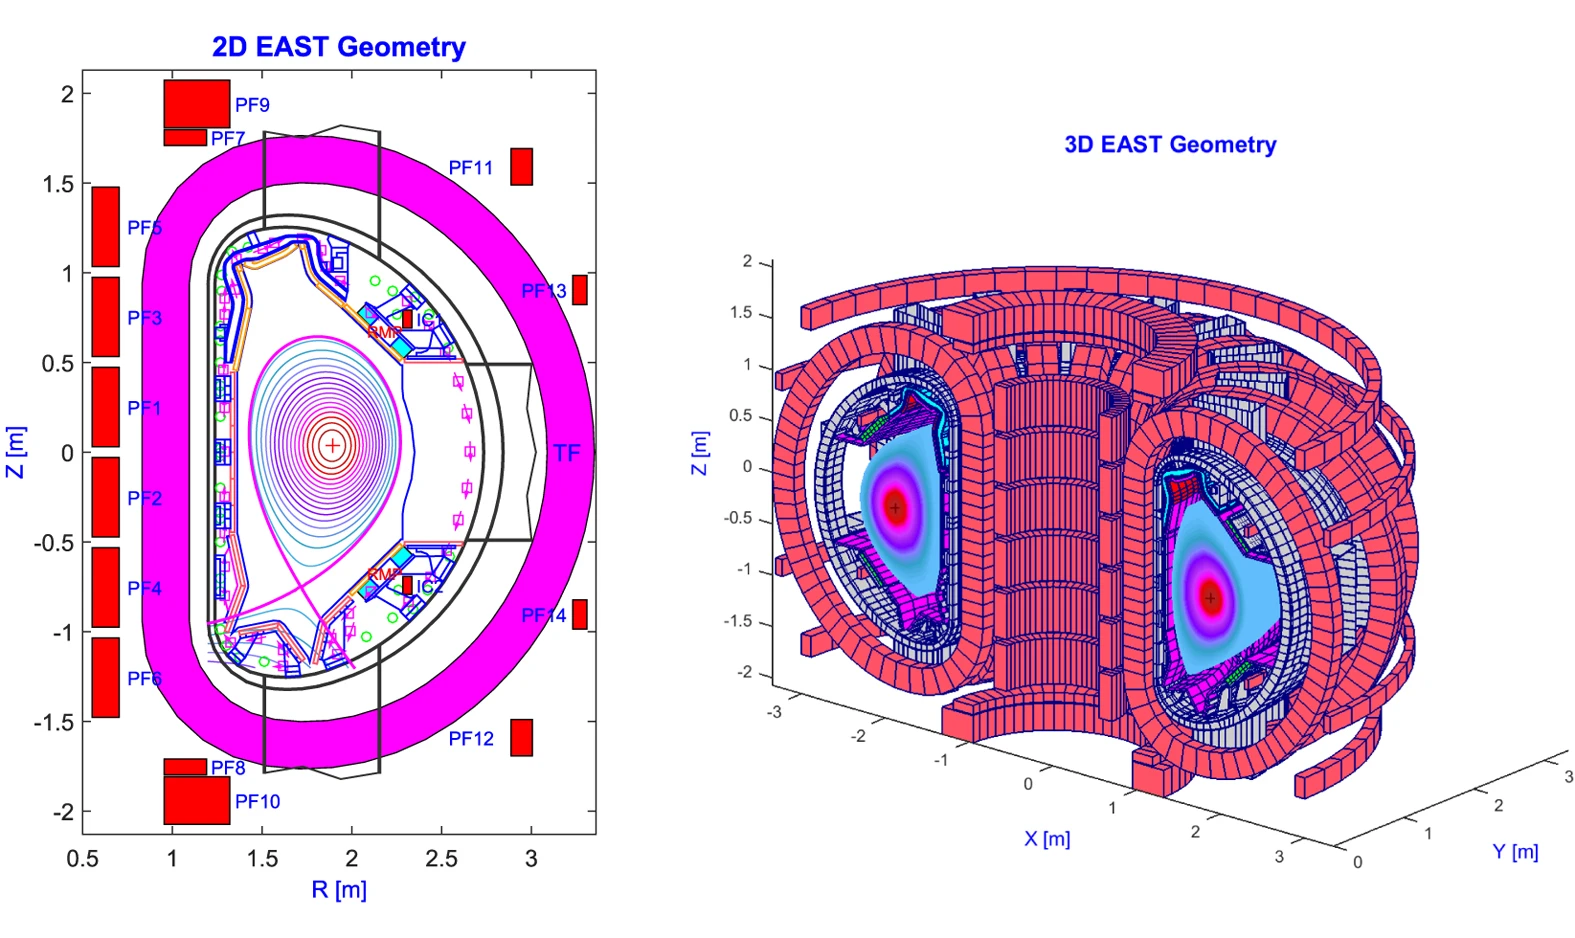
\includegraphics[scale=0.2]{imgs/c1/east-cross-section.png}
    \caption{EAST fusion reactor geometry. This is a 3D model of its cross section, highlighting the irregular shape \cite{east-geometry-article}}
    \label{fig:east-geometry}
\end{figure}

Diagram

Poloidal vs toroidal flux

Magnet positioning

Heating of plasma

Confinement

REs

% 1.2
\section{What problem does this thesis address?}

Talk about paper Matthew and Artur released. Presence of residual REs.

\TODO 

\red{Much of the justification for this can just be pawned off to the background section 
for it, this can be small. Spend more time motivating why we care.}

% 1.2.1
\subsection{What results do we seek?}

To provide a theoretical basis for exploring the observed anomalies. 
To see if theory supports the observation

\TODO

% 1.3.
\section{Project Progression}

I began this project by first doing a lot of reading. Without a formal phsyics education past grade 12, it was 
important to develop an understanding for the underlying processes that are happening so as to ensure an understanding 
of the mathematics we deal with. Additionally, much of the mathematics I encountered was new to me. For example, until this thesis, I had 
not come across the definition of a PDE before, let alone reasoned about a solution to one and used it to run a simulation. Regardless, 
the very first step of the process was to read - that began with Wesson's classic textbook "Tokamaks", accompanied by a series of lectures 
given by Matthew Hole at ANU for a fusion science special topics course delivered in 2022, and branched from there.

The inspiration for this thesis (as we stated in the section above, and will frequent throughout the thesis) was a paper 
published by Artur Malaquias and Matthew Hole, "Experiments during AC current transition in ISTTOK and the hypothesis of ballistic 
runaway electrons" \cite{malaquias-matthew}.

\TODO

Work inspired by Matthew's paper 

First expanded MHD equations linearly with a perturbation treatment

Mathematical PDE theory developed by Wang. Identified errors in paper, fixed. 

Developed a simulation to reproduce results. Then went other direction, 
solving for parameters for data. 

Simulated current inversion.

ISTTOK data matching.

Feasibility.



% 1.4.
\section{Structure of Thesis}

\TODO (after writing it)

  
\chapter{Background}
\label{chapter2}

% 2.1
\section{Magnetohydrodynamics}


The term ``magnetohydrodynamics'' (MHD) is a portmanteau of two physical concepts which are used to model plasmas 
inside fusion reactors: the ``magneto'' term comes from ``magnetic field'', and ``hydrodynamics'' indicates a 
a fluid dynamics component. Put together, magnetohydrodynamics is the study of electrically conductive materials 
that behave like fluids. Essentially it provides a way to model the behaviour of a (considerably volumous!) 
mass of particles, and their electrodynamic forces, as if it were a fluid, as opposed to having to model 
individual particle interactions. This idea was first introducd by Hannes Alfv\'en in 1970, for which he earned 
the Nobel prize \cite{alfven-mhd}!

Much modern research uses some variation of an MHD model (and the derived Grad-Shafranov Equation, which we will 
soon be introduced to) for a number of reasons, not least being its comparative computational efficiency.
One primary benefit of treating our plasma as a fluid being that we avoid modelling the behaviour of 
each individual particle in said plasma, a simplification which becomes especially important when we consider 
the order of number of particles we would have to simulate is of order $\sim 10^{20}$ - far too much 
for the author's ThinkPad to even contemplate!

Here we will build the relevant MHD background for this thesis, deriving the MHD equations from first principles, 
and explaning the assumptions we make to reduce them to a simplified state known as ``ideal MHD''. From there we will 
look at the PDE which models the behaviour of a plasma inside a Tokamak, the ``Grad-Shafranov Equation''. We will 
then note some pitfalls of using this model to describe AC configuration Tokamaks (as we are investigating), 
and finish with a discussion on runaway electrons (RE).

% 2.1.1.
\subsection{MHD Theory}

Given MHD is the marriage of fluid dynamics with electrodynamics, it is only natural to begin our 
study looking at the equations which describe electrodynamic behaviour --- Maxwell's equations 
describe the interaction between magnetic fields $\vec{B}(\vec{r}, t)$, electric fields $\vec{E}(\vec{r}, t)$, and 
the current density $j(\vec{r}, t)$ which induces them, where $\vec{r} \in \R^3$ is a position vector and $t \in \R$ describes time. Thus, we introduce Maxwell's equations:
\begin{definition}
    Maxwell's equations are given \cite{wesson-tokamaks}:
    \begin{align}
        \nabla \times \vec{B} &= \mu_0 j + \frac{1}{c^2} \pdv{\vec{E}}{t} \\
        \nabla \times E &= -\pdv{\vec{B}}{t} \\
        \nabla \cdot \vec{B} &= 0 \\
        \nabla \cdot E &= \frac{\rho_c}{\epsilon_0}
    \end{align}

    The functions driving change in this system are $\rho_c(\vec{r}, t)$, the electric charge density, and $j(\vec{r}, t)$, 
    the electric current density. We also have $\mu_0$, the free-space magnetic permeability (in henry $m^{-1}$); $\epsilon_0$, 
    the free-space permittivity; and $c$, the speed of light.
    
\end{definition}

These equations give us a way to reason about the electric and magnetic fields if we're given some descriptor for the 
current we're passing through some medium. We are now to introduce the fluid dynamics component to our system. A fluid's 
mass density can be given by summing over the effects of individual ``species'' of particles (e.g. electrons) in the fluid:
$$\rho_c = \sum_{\sigma} m_{\sigma} n_{\sigma}$$
and its current density similarly:
$$\vec{j}(\vec{r}, t) = \sum_{\sigma} n_{\sigma} q_{\sigma} \vec{u}_{\sigma}$$
where $\sigma$ describes a particle species, $m_\sigma$ describes its mass, $n_\sigma$ its number density 
(a measurement of concentration for the given particle species in a pre-defined volume -- akin to Avogadro's constant), 
$q_\sigma$ describes its electric charge, and $\vec{u}_\sigma$ the mean velocity of this species of particle in the fluid. 

\subsubsection{Fluid Dynamics}

\begin{notn}
    A common simplification in notation for fluids is made in using the \emph{Lagrangian derivative}, given:
    $$\frac{\DD}{\DD t} = \left (\pdv{t} + \vec{u} \cdot \nabla \right )$$ 
    It describes the total change in a volume within a fluid as it moves throughout said fluid. It is essentially 
    a change in reference frame for a derivative - where a regular derivative might descirbe, for example, 
    how a particle moves with respect to time in its surroundings, its Lagrangian will take into account 
    the motion of the fluid the particle is immersed in as well.
\end{notn}

We begin with conservation of mass, also known as the ``continuity equation''. 

\begin{definition}[The continuity equation]
    The below relates how mass density, $\rho$, changes with respect to the motion of a 
    fluid element.

    \begin{equation}
        \pdv{\rho}{t}  = -\nabla \cdot \left ( \rho \vec{u} \right ) \label{continuity}
    \end{equation}

    The derivation of the above comes from a surface integral over a volume with an outward and inward flux, 
    and an application of Gauss' flux law. For a full derivation, see pg. 19 - 21 of \cite{mhd-lectures}.
\end{definition}

\begin{remark}
    The above is a PDE with four variables: $\rho$, the mass density of the medium, and $\vec{u}$, the velocity 
    of the fluid. This renders the system not closed, and thus too general for an analytic solution - we have 
    more unknowns than we have equations \cite{mhd-lectures}. Later we 
    will introduce other equations to our system to apply more restrictions, and make assumptions about the 
    physicality of the system which will reduce these dependencies, and make it determined (``closed'').
\end{remark}

\begin{remark}
    We can rewrite \eqref{continuity} with a Lagrangian frame of reference, as 
    \begin{align}
        &\frac{\DD}{\DD t}\rho = -\rho \nabla \cdot \vec{u} \\
        \iff &\frac{\DD}{\DD t}\rho + \rho \nabla \cdot \vec{u} = 0 \label{continuity-lag}
    \end{align}
\end{remark}

Equation \eqref{continuity} (and equivalently \eqref{continuity-lag}) tells us that the mass of our fluid is conserved for motion of a volume element 
of our fluid - one assumption we make for our model. Next we'll discuss fluid motion as described by Newton for a fluid element:

\begin{definition}[Newtonian Fluid Motion]
    Newton's law for a fluid specifies:
    \begin{align}
        \rho \frac{\DD }{\DD t} \vec{u} &= \vec{F}
    \end{align}
    where $\rho(\vec{r}, t)$ is the mass density of the fluid, 
    $\vec{u}(\vec{r}, t)$ describes the velocity of the fluid element, and $\vec{F}(\vec{r}, t)$ 
    describes the force per unit volume acting on the fluid element \cite{mhd-lectures}.
\end{definition}
The forces acting on particles within a fluid can be split into two types
\begin{itemize}
    \item Gravitational
    
    Here, $\vec{F}_g = \rho \vec{g}$, where $\vec{g}$ is the gravitational acceleration. This should hark back to high school 
    physics, though note this is a vector here as we care about the direction gravity accelerates the fluid element in, 
    and relativistic effects can be an important consideration for high mass systems. This is more relevant for cases that 
    you are using the MHD equations to describe the dynamics of large systems, such as a star. Unsurprisingly, this is less relevant 
    for our case of plasmas within relatively miniscule Tokamaks.

    \item Electromagnetic
    
    This is the interesting part for us. As we assume our fluid is capable of conducting electricity (it's a plasma after all),
    there are electromagnetic forces operating within the fluid that affect the behaviour of the particles that the fluid consists of. 
    The electromagnetic forces themselves can be split into two types, the \textbf{electric force} given by $\vec{F}_q = \rho_c \vec{E}$, 
    and the \textbf{Lorentz force}, given $\vec{F}_{L} = \vec{j} \times \vec{B}$ (where $\vec{B}(\vec{r}, t)$ describes the magnetic field)
\end{itemize}
Taking these forces into account, we can describe the motion of an element of our fluid moving with velocity $\vec{u}$ 
via:
\begin{equation}
    \rho \frac{\DD}{\DD t} \vec{u} =  \vec{j} \times \vec{B} + \rho_c \vec{E} - \nabla p + \rho \vec{g}
\end{equation}


\begin{remark}
    Here the $\rho \vec{g}$ term could be abstracted further away into a stress tensor, as described by equation 4.20 of \cite{mhd-lectures}. These 
    pressures however are largely negligible when dealing with the scale we do in Tokamak plasmas however, and 
    are thus ignored. We will soon drop the gravitational consideration as well anyway, but include it here for now for completeness.
\end{remark}

\begin{remark}
    The equation we have introduced is a function of six variables in its complex form (with stress tensor 
    included), though even in this form we still have more variables than we do equations (1). Similar to before, this 
    is not constrained sufficiently to consider it a closed system.
\end{remark}

We next relate a plasma's pressure to its motion. We will simply present it here, though important notes in its 
derivation are that we assume the plasma behaves as an ideal gas (which is to say the only interaction 
between particles within the plasma are via elastic collisions with each other, or the boundaries of the container 
it is contained within). This is equivalent to saying that energy in the system depends only on the pressure. Thus, the 
energy equation is given:
\begin{definition}[Energy Equation]
    Where $\vec{p}(\vec{r}, t)$ describes the pressure of our fluid:
    \begin{equation}
        \frac{\DD}{\DD t} p  = -\Gamma p \nabla \cdot \vec{u} + (\Gamma - 1) \left [ -\nabla \cdot \vec{q} + \vec{\Pi} : \nabla \vec{u} + \eta \vec{J}^2 \right ]
    \end{equation}
    where $\Gamma$ describes ``abiabatic index'' (a known constant for plasmas), $q$ is the heat flux through 
    the boundary of the volume; $\eta$ is the electrical resistivity of the fluid; and $\vec{\Pi}$ is the viscous 
    stress tensor (the component which we replaced with $\rho \vec{g}$ earlier), and will soon ignore again. 
\end{definition}



The equations we've looked at constitute what are known as the fluid equations:

\begin{definition}[Fluid Equations]
    \begin{align}
        \frac{\DD}{\DD t} \rho &+ \nabla  \cdot \rho \vec{u} = 0 \\
        \rho \frac{\DD}{\DD t} \vec{u} &=  \vec{j} \times \vec{B} + \rho_c \vec{E} - \nabla p + \rho \vec{g} \\
        \frac{\DD}{\DD t} p  &= -\Gamma p \nabla \cdot \vec{u} + (\Gamma - 1) \left [ -\nabla \cdot \vec{q} + \vec{\Pi} : \nabla \vec{u} + \eta \vec{j}^2 \right ]
    \end{align}
\end{definition}

As reiterated a couple times now, these equations form an unclosed system, and are thus undetermined. 
To resolve this we introduce some constraints that come from electrodynamic forces, and a couple other 
relations that lead to a closed system.

\subsubsection{Electrodynamics}

As it currently stands, the input variables for the fluid equations are $\rho(\vec{r}, t)$ and $p(\vec{r}, t)$. We note that 
the electric field $\vec{E}$ and the magnetic field $\vec{B}$ are generated by the electric charge density, $\rho_c$, and 
the current density $\vec{j}$. This is where Maxwell's equations come into play. By combining Maxwell's equations with the 
fluid equation given above, we achieve the MHD model. The only piece to our puzzle missing is to tie the motion of the fluid 
(through $\vec{u}$) to the behaviour of the electric and magnetic fields. This is done via \textit{Ohm's} law:
\begin{equation}
    \vec{E} + \vec{u} \times \vec{B} = \eta \vec{j}
\end{equation}
\begin{remark}
    Note that the above is technically a lie, as it does not take into account relativistic effects, though for simplicity 
    our MHD model ignores these.
\end{remark}


\begin{definition}[MHD Equations]
    The MHD equations can then be summarised:
    \begin{align}
        \frac{\DD}{\DD t} \rho &= 0 \\
        \rho \frac{\DD}{\DD t} \vec{u} &= -\nabla p + \vec{j} \times \vec{B} + \nabla \cdot \Pi \\
        \frac{\DD}{\DD t} p  &= -\Gamma p \nabla \cdot \vec{u} + (\Gamma - 1) \left [ -\nabla \cdot \vec{q} + \vec{\Pi} : \nabla \vec{u} + \eta \vec{j}^2 \right ] \\
        \pdv{\vec{B}}{t} &= -\nabla \times \vec{E} \\
        \mu_0 \vec{j} &= \nabla \times \vec{B} \\
        \vec{E} + \vec{u} \times \vec{B} &= \eta \vec{j}
    \end{align}
\end{definition}

\begin{remark}
    The MHD equations as presented above constitute 14 equations with 27 unknowns. The breakdown is as such:
    \begin{itemize}
        \item $\rho$ : 1 unknown
        \item $\vec{u}$ : 3 unknowns
        \item $p$: 1 unknown
        \item $\vec{\Pi}$ : 9 unknowns
        \item $\vec{j}$ : 3 unknowns
        \item $\vec{B}$ : 3 unknowns
        \item $\vec{E}$ : 3 unknowns
        \item $\vec{q}$ : 3 unknowns
        \item $\eta$ : 1 unknown
    \end{itemize}
\end{remark}

The above is obviously insufficiently constrained for purposes of identifying a solution. We will skip a large amount 
of the work required to reduce the above to a closed system, though for details see lecture 7 of \cite{mhd-lectures}. 
For now, we will comment on two reduced MHD models:

\subsubsection{Resistive MHD}
The resistive MHD model comes about by setting $\vec{q} = 0$ and $\vec{\Pi} = 0$. Here, we have $\eta \ne 0$ notably. The model 
is given:
\begin{definition}[Resistive MHD]
    \begin{align}
        \frac{\DD}{\DD t} \rho &= 0 \\
        \rho \frac{\DD}{\DD t} \vec{u} &= -\nabla p + \vec{j} \times \vec{B}\\
        \frac{\DD}{\DD t} p  &= -\Gamma p \nabla \cdot \vec{u} \\
        \pdv{\vec{B}}{t} &= -\nabla \times \vec{E} \\
        \mu_0 \vec{j} &= \nabla \times \vec{B} \\
        \vec{E} + \vec{u} \times \vec{B} &= \eta \vec{j}
    \end{align}
\end{definition}

\begin{remark}
    The most notable effect of resistive MHD is that allowing for electrons to diffuse allows the resulting magnetic field lines 
    to reconnect, which leads to breaks in the magnetic field line topology. This can lead to the generation of fast particles, i.e., 
    runaway electrons.
\end{remark}


\subsubsection{Ideal MHD}
The ideal MHD equations are one step removed from the resistive MHD model --- in fact they are equivalent, only for the ideal MHD case 
we also ignore resistivity. Thus, set $\eta = 0$, and we obtain the ideal MHD equations:
\begin{definition}[Ideal MHD]
    \begin{align}
        \frac{\DD}{\DD t} \rho &= 0 \\
        \rho \frac{\DD}{\DD t} \vec{u} &= -\nabla p + \vec{j} \times \vec{B}\\
        \frac{\DD}{\DD t} p  &= -\Gamma p \nabla \cdot \vec{u} \\
        \pdv{\vec{B}}{t} &= -\nabla \times \vec{E} \\
        \mu_0 \vec{j} &= \nabla \times \vec{B} \\
        \vec{E} + \vec{u} \times \vec{B} &= 0
    \end{align}
\end{definition}

\begin{remark}
    In doing this, we have removed the dependency on $\vec{\Pi}$, $\eta$ and $\vec{q}$, which accounts 
    for 13 unknowns. This brings the total number of equations to 14 (or $8$ if you make a substitution 
    for Ohm's law) with 14 ($8$) unknowns. Thus, under the ideal MHD model, the system is closed.
\end{remark}


\red{Brief discussion on what resistivity is?}
\red{Tie into GSE}
% 2.2. 
\section{Grad-Shafranov Equation}

What is it

What do its components describe

Solutions to GS equation?

% 2.2.1
\subsection{Derivation}

Go through derivation of it 

% 2.3.
\section{AC Configuration Tokamaks}

Tokamak's normally in DC mode. What does it mean for a fusion reactor 
to operate in AC mode

% 2.3.1.
\subsection{Physical Differences}

Plasma current (talk: operation of toroidal coils to regulate current)



% 2.3.2.
\subsection{Why Bother?}

What benefits are there to using an AC design over DC?

Talk about confinement time, stability, etc

% 2.4
\subsection{Runaway Electrons}

\subsubsection{Generation Mechanisms}

Here we will discuss how runaway electrons come to exist within a Tokamak's fusion cycle.

\subsubsection{RE Detection}

\subsubsection{Why we care}


  
\chapter{Current Reversal Theory}
\label{chapter3}



% 3.1.
\section{Perturbation Methods}

% 3.1.1.
\subsection{What is a Perturbation Treatment?}

When it comes to solving differential equations, the ideal scenario 
is that you find an analytic solution, $\psi$. This, however, is generally a 
difficult problem, and especially so in the case of differential equations. A great deal 
of research goes into trying to find analytic solutions to PDEs, 
which is no less true for the Grad-Shafranov equation and its variations. Though 
such efforts are often futile, or require making assumptions about properties of 
your solution which may not be representative of what you're trying to show, 
other means of obtaining the $\Psi(\vec{x})$ for $\vec{x} \in \Omega$ have been developed.

A traditional approach to this is to use some numerical code to approximate solution values. 
There are various codes which exist for this purpose specifically with regards to 
the GSE equation, such as SPEC \cite{spec-code}. These codes come in many flavours - 
some implement a particle simulation, which can provide precision with simulation, 
though are computationally costly. Others exploit various properties of the 
variant of GSE they target and may be computationally more feasible, but are 
restricted in scope, application, and/or reliability because of their assumptions.

A common problem that numerical methods seek to solve is that of time evolution. 
Simulations which evolve a system through time, for obvious reasons, do not discard 
the time dependency component in their derivation of the GSE. 
A common problem that numerical methods are employed to solve is that of time evolution. 
Simulations which evolve a system through time however often require time dependence in the 
system they are trying to solve -- something, if you recall from our derivation of the GSE, is 
not present in our model. This introduces a difficulty for us, as solutions to the GSE explicitly 
represent plasma equilibria, and so we expect no variation of the system with respect to time.

For this thesis, given the availability of an analytic solution to a variation of 
the GSE that specifically relates to current reversals, we employ a hybrid approach. 
In our simulation we wish to observe changes in the system through a current ramp down
- this necessitates a time dependency component to our solution. However, there are 
a couple points to note:
\begin{itemize}
    \item Time evolution simulations are expensive
    \item Existing literature on time evolution GSE do not take into account the possibility for current 
    reversal
    \item The GSH variant we utilise (which has yet to be introduced) is not time dependent, i.e., 
    was not derived taking into account a time component
\end{itemize}

There are a couple possible avenues we could explore from here. We could implement a numerical code 
for the time evolution, for example a particle simulation, however this is for all intents and purposes
computationally infeasible given the hardware available (a beloved but dilapidated Thinkpad T440p). We could 
attempt to find an analytic solution to the GSE with time dependence (or an approximation to one),
but given the mountain of research existing in this space and the relative inexperience 
of the author, this would likely be a futile task. The third, and most lucrative option, 
is to use an existing analytic solution to a variation of the GSE that accounts for 
current reversal, and explore if small changes to its state
are sufficiently ``good enough'' approximations of our system that it can be used to make 
statements about experimental data.

This is where perturbation theory comes in. Intuitively we would expect a 
plasma to vary ``smoothly'' - nature rarely behaves in instantaneous ways. The 
analytic solution we will soon have describes the instantaneous state (a slice in time) of 
our plasma's state. We may anticipate then that if we were to change something 
in our system by a ``sufficiently small amount'' (we will later comment on what exactly is meant by sufficiently small), 
that our system may react to that change of state in a way that approximates how it would if it 
were really varying through time. 

\subsubsection{Resistivity Note}
When we derived the ideal MHD equations we compared them to the resistive MHD model, noting that 
the removal of resistivity would be an important simplification to note. Here we see its importance, as 
we are now allowing our system to vary with respect to time, which means that there exists some time scale 
for which resistive effects will begin to impact the behaviour of our plasma. 

Our model assumes the ideal MHD assumptions however, which includes dropping resistivity, and so the effect 
of these resistive instabilities is lost in our model. The question of whether these effects are significant 
enough to affect the accuracy of our time evolution is one we hope to answer when we come to reviewing our simulations in 
chapter \ref{chapter5}.

A perhaps more intuitive analogy is that of swimming. Imagine you are stationary sitting 
at the bottom of a pool, and you are looking at your arm extended out in front of you. 
Focus on the feeling of the water moving around your arm - this will emulate the resistivity 
that electrons would feel. If you move your arm abruptly, 
perhaps in a cutting motion, then you will feel the pressure of the water push against 
your arm, and that might affect how quickly you can move your arm, or if the current of the water is 
particularly strong, perhaps you notice your arm move not in the direction you intended. Perhaps 
you also have to use more energy to move your arm than you intended, so it doesn't go as far. 
Now imagine instead that you don't abruptly cut, but instead, very slowly, almost 
imperceptibly, move your arm through the water. In this case you may not be aware of any resistance at all 
- there is no sensation of resistance, your arm moves exactly as fast as you expect it to, and you use exactly 
the amount of energy to move it as you expected. However, if you do this for long enough, perhaps you 
will begin to notice the effects more and more. Or maybe by now you'll realise you're out of breath and need 
to resurface. An instructive graphic is below.

\begin{figure}[h!]
    \centering
    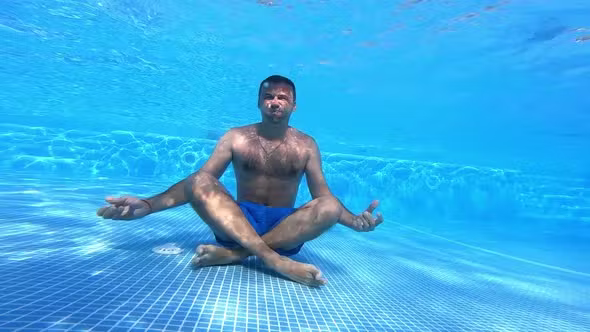
\includegraphics[scale=0.6]{imgs/c3/pool.png}
    \caption{Demonstrative graphic for conducting a resistivity experiment at the bottom of a pool.}
\end{figure}
\newpage

We will have the ability to determine the 
state of our system for some given parameters, and so the question becomes: can 
we vary our input in a way such that the behaviour of the analytic solution to 
the GSH is an approximation of a time evolution of the plasma. We are able to compare 
our results to experimental data, and then exploit our work to answer further questions.



% 3.1.2.
\subsection{Regular Perturbation Theory}

At the heart of perturbation theory is the manipulation of functions by some small amount to achieve a goal. A familiar 
perturbation is the taylor expansion - if we have some function $f(x)$, then we can use $n^{\text{th}}$ order derivatives to approximate 
the value of the function for some perturbation $a$
\begin{equation*}
    f(x) = \sum_{n = 0}^{\infty} \frac{f^{(n)}(a)}{n!} (x - a)^n
\end{equation*}
In a similar spirit, we can expand a function $f(x)$ around a point $x = a$ by some $\epsilon$ amount
$$f(a + \epsilon) = f(a) + \epsilon \dv{f}{x}(a) + \frac{1}{2} \epsilon^2 \dv[2]{f}{x}(a) + \dots$$
and it is this sentiment that drives perturbation theory - that some small change in input of a function can result 
in small changes in the output of that function. This is obviously not the case for all functions - immediately we see that this 
fails for anything that is not differentiable, and in general if we wish to make an approximation to the $n^{\text{th}}$ degree then 
we need our function to at least be $f \in C^n$ \cite{perturbation-basics}. 

When it comes to PDEs, regular perturbation theory can be used to find solutions to unknown functions. The general process is \cite{perturbation-basics}:
\begin{enumerate}
    \item Set $\epsilon = 0$, solve the resulting system (i.e., a solution for $f_0$ effectively)
    \item Perturb the system by $\epsilon$ (i.e., go back and expand the system in terms of some $\epsilon > 0$)
    \item Let the (unknown) solution to the new perturbed system be given as
    $$f_0 + \epsilon f_1 + \epsilon^2 f_2 + \dots$$
    \item Expand the PDE in terms of $\epsilon$. Collect like powers of $\epsilon$ and solve these as their own systems
    \item Collate solutions for each $f_i$ as found for their respective powers of $\epsilon$ - this is your approximation 
    to the analytic solution to the PDE
\end{enumerate}

\noindent
Formally then we can state that, given a differential equation
$$F(D^{k} u(x), D^{k-1}u(x), \dots, Du(x), x) = 0$$
an expansion for $u$ can be given
$$u(x) = u_0(x) + \epsilon u_1(x) + \epsilon^2 u_2(x) + \dots$$
If we were able to reason about all the derivatives of $u$ (and they exist), then in the ideal case we 
can retrieve an analytic solution to the PDE. However, if instead the function is not $C^{\infty}$, or perhaps 
becomes too difficult to analytically solve, we could instead solve for an approximate solution by instead expanding, for 
example, to the second order:
$$u(x) = u_0(x) + \epsilon u_1(x) + \epsilon^2 u_2(x) + \mathcal{O}(\epsilon^2)$$

\subsubsection{Example}
Here we will follow an example provided by \cite{perturbation-example}, which emphasis the utility of perturbation methods in solving 
differential equations. 

Let a body have mass $m$ with initial velocity $v_0$. It moves in a straight line, however there is a resistive force opposing its motion 
with magnitude $av - bv^2$, where $v(\tau)$ describes the velocity of the object. We assume $b \ll a$ are constants, and Newton's law provides
$$m \dv{v}{\tau} = -av + bv^2$$
with the boundary condition
$$v(0) = v_0$$
We can make this system dimensionless by making a change of variables with $y = v / v_0$ and $t = \tau / (m / a)$, giving us the new system
$$\dv{y}{t} = -y + \epsilon y^2$$
with boundary condition
$$y(0) = 1$$
where $\epsilon \equiv (b v_0) / a \ll 1$. Now with our dimensionless model we can begin our perturbations. 
Instead of opting for an analytic solution, 
we'll use an approximation, so we will expand as such:
$$y(t) = y_0(t) + \epsilon y_1(t) + \epsilon^2 y_2(t)$$
and ignore any $\mathcal{O}(\epsilon^3)$ terms. Substituting this into our dimensionless model gives
\begin{align*}
    \dv{y}{t} &= -y + \epsilon y^2 \\
    y_0' + \epsilon y_1' + \epsilon^2 y_2' &= -(y_0 + \epsilon y_1 + \epsilon^2 y_2) + \epsilon \left (y_0 + \epsilon y_1 + \epsilon^2 y_2 \right )^2
\end{align*}
Then, we next collect similar powers of $\epsilon$ (representing different orders of approximation), which we observe is a series of 
linear ODEs:
\begin{align*}
    y_0' &= -y_0 \\
    y_1' &= -y_1 + y_0^2 \\
    y_2' &= -y_2 + 2y_0 y_1
\end{align*}
The initial condition also tells us that $y_0 (0) + \epsilon y_1(0) + \epsilon^2 y_2(0) = 1$, but, as we know $y_0(0) = 1$, 
we also get that $y_1(0) = y_2(0) = 0$. Thus, we have a series of ODEs with initial conditions specified for each, which 
harks back to first year calculus courses. We readily have solutions available for each of the ODEs:
\begin{align*}
    y_0(t) &= e^{-t} \\
    y_1(t) &= e^{-t} - e^{-2t} \\
    y_2(t) &= e^{-t} - e^{-2t} + e^{-3t}
\end{align*}
and thus, our approximate solution to $y$ can be given
$$y(t) \approx e^{-t} + \epsilon(e^{-t} - e^{-2t}) + \epsilon^2 (e^{-t} - e^{-2t} + e^{-3t})$$
As a form of validation, with omnipotent knowledge we can state that the actual solution to the original equation can 
be given as 
$$y(t) = \frac{e^{-t}}{1 + \epsilon(e^{-t} - 1)}$$
which has the Taylor series expansion (in $\epsilon$):
$$y(t) = e^{-t} + \epsilon(e^{-t} - e^{-2t}) + \epsilon^2(e^{-t} - e^{-2t} + e^{-3t}) + \mathcal{O}(\epsilon^3)$$
which is exactly what our perturbation approximation determined \cite{perturbation-example}. A cool demonstration, if we can say so ourselves!

While we won't be performing such an in depth perturbation treatment of the MHD equations themselves, it is this spirit 
of approximation via perturbation which we will carry through our work, and keep in mind when it comes to our simulations.

% 3.1.3.
\subsection{Ideal MHD Perturbation}

At the beginning of this thesis we introduced it as being interdisciplenary in nature. 
Keeping in that spirit, at times here we will put on our physicists cap and 
seemingly arbitrarily remove terms we no longer wish to have. We 
kindly ask that any mathematicians reading these sections avert their gaze in such 
times so as to maintain sanity.

In chapter \ref{chapter2} we derived the ideal MHD equations, and their subsequent reduction used in GSE, given:
\begin{align}
    \vec{j} \times \vec{B} &= \nabla p \\
    \mu_0 \vec{j} &= \nabla \times \vec{B} \\
    \nabla \cdot \vec{B} &= 0
\end{align}
These by note are time independent. We wish to look at the 
effect of some small ($\epsilon > 0$) time perturbation to the original system however, and so 
will return to their derivation, this time without discarding the time component. Consider the pre-GSE ideal MHD equations again, 
as given in (\eqref{ideal-mhd-first} - \eqref{ideal-mhd-last})
\begin{align*}
    \frac{\DD}{\DD t} \rho &= -\rho \nabla \cdot \vec{u} \\
    \rho \frac{\DD}{\DD t} \vec{u} &= -\nabla p + \vec{j} \times \vec{B}\\
    \frac{\DD}{\DD t} p  &= -\gamma p \nabla \cdot \vec{u} \\
    \shortintertext{with the assumptions}
    \pdv{\vec{B}}{t} &= -\nabla \times \vec{E} \\
    \mu_0 \vec{j} &= \nabla \times \vec{B} \\
    \vec{E} + \vec{u} \times \vec{B} &= 0 
\end{align*}

We will apply our perturbation treatment to the first two equations of these (the continuity equation, momentum equation), 
using the assumptions to aid us. We will begin with the continuity equation.

\subsubsection{Continuity Equation Time Perturbation}
We restate the continuity equation:
\begin{equation*}
    \frac{\DD}{\DD t} \rho = -\rho \nabla \cdot \vec{u}
\end{equation*}
Here we have two functions, $\rho$ and $\vec{u}$, which are both functions of three dimension in space and one of time, i.e.
\begin{align*}
    \rho &:= \rho(\vec{r}, t) \\
    \vec{u} &:= \vec{u}(\vec{r}, t)
\end{align*}
where $\vec{r} \in \R^3, t \in \R$. Here (and throughout these perturbation treatments) we will decouple the time dependency by 
assuming it to be some epsilon perturbation from an initial state. For example, for mass density ($\rho$), we can let $\rho_0$ 
describe some initial state that is only dependent on space, and $\rho_1$ a perturbation component similarly dependent only on space. Let $\epsilon_{\rho} > 0$ be some small perturbation factor
for mass density, and $t$ be the time evolved for. Then we prescribe a time-linear perturbation expansion as such:
\begin{align*}
    \rho(\vec{r}, t) &= \rho_0(\vec{r}) + \epsilon_\rho t \rho_1(\vec{r}) + \mathcal{O}(\epsilon_\rho^2)
    \shortintertext{and analogously:}
    \vec{u}(\vec{r}, t) &= \vec{u}_0(\vec{r}) + \epsilon_u t \vec{u}_1 (\vec{r}) + \mathcal{O}(\epsilon_u^2)
\end{align*}
Here the $t$ term effectively acts as a scaling factor on top of $\epsilon$. We have also dropped any $\epsilon$ terms of order 
greater than $1$ in our approximation, that is to say, if we were to be accurate our expansion would actually be:
\begin{align*}
    \rho(\vec{r}, t) &= \rho_0(\vec{r}) + \epsilon_\rho t \rho_1(\vec{r}) + \epsilon^2_\rho t \rho_2(\vec{r}) + \dots \\
    \vec{u}(\vec{r}, t) &= \vec{u}_0(\vec{r}) + \epsilon_u t \vec{u}_1 (\vec{r}) + \epsilon^2_{u} t \vec{u}_2(\vec{r}) + \dots
\end{align*}
As we said at the start of this chapter however, this is an interdisciplenary thesis, and the above is an example of us putting on our 
physicist cap and deciding to remove ``unnecessary'' complexity. Physically we can justify this dropping of terms as we would expect terms of 
greater order to contribute diminishingly to our system. That is to say, on the time scales we are considering, an approximation of up to $\epsilon$ 
should be sufficient for experimental comparisons. As such, we need only to reason about that, and drop any terms on order of $\mathcal{O}(\epsilon^2)$.
We substitute these perturbation expansions into our equation. For brevity we will drop function parameters in our notation, and 
first begin with an expansion of the $\rho$ term:
\begin{align*}
    \shortintertext{\textit{LHS:}}
    \frac{\DD}{\DD t} \rho &= \left ( \pdv{t} + \vec{u} \cdot \nabla \right ) \rho \\
    &= \pdv{t} \rho + \vec{u} \cdot (\nabla \rho) \\
    &= \pdv{t} (\rho_0 + \epsilon_\rho t \rho_1) + \vec{u} \cdot (\nabla (\rho_0 + \epsilon_\rho t \rho_1)) \\
    &= \pdv{t}\rho_0 + \epsilon_\rho \rho_1 + \vec{u} \cdot (\nabla \rho_0) + \epsilon_\rho t \vec{u} \cdot (\nabla \rho_1) \\
    \shortintertext{noting that $\rho_0$ is not a function of time}
    &= \epsilon_\rho \rho_1 + \vec{u} \cdot (\nabla \rho_0) + \epsilon_\rho t \vec{u} \cdot (\nabla \rho_1)
    \shortintertext{\textit{RHS:}}
    -\rho \nabla \cdot \vec{u} &= -(\rho_0 + \epsilon_\rho t \rho_1) (\nabla \cdot \vec{u}) \\
    &= -\rho_0 (\nabla \cdot \vec{u}) - \epsilon_\rho t \rho_1 (\nabla \cdot \vec{u})
\end{align*}
\begin{align*}
    \shortintertext{\textit{Combined:}}
    \frac{\DD}{\DD t} \rho &= -\rho \nabla \cdot \vec{u} \\
    \epsilon_\rho \rho_1 + \vec{u} \cdot (\nabla \rho_0) + \epsilon_\rho t \vec{u} \cdot (\nabla \rho_1) &= -\rho_0 (\nabla \cdot \vec{u}) - \epsilon_\rho t \rho_1 (\nabla \cdot \vec{u}) \\
    \epsilon_\rho \rho_1 + \epsilon_\rho t \left [ \vec{u} \cdot (\nabla \rho_1) + \rho_1 (\nabla \cdot \vec{u}) \right ] &+ [\rho_0 (\nabla \cdot \vec{u}) + \vec{u} \cdot (\nabla \rho_0)] = 0 \\
    \epsilon_\rho \rho_1 + \nabla \cdot (\rho_0 \vec{u}) + \epsilon_\rho t [\nabla \cdot (\rho_1 \vec{u})] &= 0
\end{align*}
Here we have used the divergence property $\nabla \cdot (f\vec{v}) = (\nabla f) \cdot \vec{v} + f(\nabla \cdot \vec{v})$. Note that for the 
Grad-Shafranov equation we usually (and we shall) assume an incompressible fluid, which mathematically is significant as it gives us the property 
that $\nabla \cdot (\rho \vec{u}) = 0$. From the above we immediately get that $\epsilon_\rho \rho_1 = 0$, which just tells us that the time component 
we introduced has no effect on the system, given the assumptions we make. This is excellent news for us, as it means that small perturbations 
in our system in a manner that emulates a time evolution should not affect the accuracy of our model, at least insofar as the effects of the 
continuity equation are concerned, and up to a term of $\mathcal{O}(\epsilon^2)$. To be confident that we can do this for the Grad-Shafranov equation on a whole, we need to repeat this process for 
the other ideal MHD equations. Next we'll look at the momentum equation.

\subsubsection{Momentum Equation}
We restate the momentum equation here:
\begin{equation*}
    \rho \frac{\DD}{\DD t}\vec{u} = -\nabla \rho + \vec{j} \times \vec{B}
\end{equation*}
We will follow the same process as we did for the continuity equation. Here we have four equations, however, by introducing one of 
our GSE assumptions we can reduce this to three immediately. For GSE we assume that our fluid has no velocity, i.e. $\vec{u} = 0$, which 
gives us that $\frac{\DD}{\DD t} \vec{u} = 0$. Thus the equation we actually have to expand is:
\begin{equation*}
    0 = -\nabla \rho + \vec{j} \times \vec{B}
\end{equation*}
The three equations we have are each functions of $\vec{r} \in \R^3$ and $t \in \R$, and can be linearly perturbed in time as we did earlier. As such:
\begin{align*}
    \rho(\vec{r}, t) &:= \rho_0(\vec{r}) + \epsilon_\rho t \rho_1(\vec{r}) + \mathcal{O}(\epsilon_\rho^2) \\
    \vec{B}(\vec{r}, t) &:= \vec{B}_0(\vec{r}) + \epsilon_B t \vec{B}_1(\vec{r}) + \mathcal{O}(\epsilon_B^2) \\
    \vec{j}(\vec{r}, t) &:= \vec{j}_0(\vec{r}) + \epsilon_j t \vec{j}_1(\vec{r}) + \mathcal{O}(\epsilon_j^2)
\end{align*}
Making these substitutions into the momentum equation:
\begin{align*}
    \nabla \rho &= \vec{j} \times \vec{B} \\
    \nabla (\rho_0 + \epsilon_\rho t \rho_1) &= \vec{j} \times (\vec{B}_0 + \epsilon_B t \vec{B}_1) \\
    (\nabla \rho_0) + \epsilon_\rho t (\nabla \rho_1) &= (\vec{j} \times \vec{B}_0) + \epsilon_B t (\vec{j} \times \vec{B}_1) \\
    (\nabla \rho_0) + \epsilon_\rho t (\nabla \rho_1) = [(\vec{j}_0 \times \vec{B}_0) + \epsilon_j t (\vec{j}_1 &\times \vec{B}_0)] + \epsilon_B t [(\vec{j}_0 \times \vec{B}_1) + \epsilon_j t (\vec{j}_1 \times \vec{B}_1)] \\
    (\nabla \rho_0) + \epsilon_\rho t (\nabla \rho_1) &= \vec{j}_0 \times \vec{B}_0 + \epsilon_j \epsilon_B t^2 (\vec{j}_1 \times \vec{B}_1)
\end{align*}
If we collate terms of like order, we get 
\begin{align*}
    \nabla \rho_0 &= \vec{j}_0 \times \vec{B}_0 \\
    \nabla \rho_1 &= \frac{\epsilon_j \epsilon_B}{\epsilon_\rho} t (\vec{j}_1 \times \vec{B}_1) 
\end{align*}
both of which look remarkably like the original momentum equation; an observation which is not to be mistaken for coincidence. Notably, when we take our 
evolution over ``small enough'' time scales, the perturbation components here disappear entirely, and we are left with the version of the 
momentum equation which is used in the regular equilibrium-state derivation of the Grad-Shafranov equation. As such, we would anticipate that 
small time perturbations associated with the effects of the momentum equation will introduce ``small'' errors in the resulting GSE solution, though 
(and as we hope to observe through experiment), hopefully imperceptibly so - as the above expansion seems to suggest.  

\subsubsection{The Other Ideal MHD Equations}
Isaac Newton is quoted as saying ``it causeth my head to ache'', which he is claimed to have said in reference to perturbation expansions 
in trying to determine the orbit of the Moon \cite{newton-headache}. Hopefully understandably, we ask that the reader excuse our omitting the working for the more involved of the ideal MHD equations, 
as to write it all down here would be to commit an expositionary crime. The expansion of the remaining equations however leads to a similar outcome 
as we found with the continuity equation and the momentum equation - that, up to an $\epsilon$ factor, the time perturbed ideal MHD equations do not show significant deviation 
from their equilibrium counterparts. 

\subsubsection{Significance}
The purpose of this exercise was to provide some theoretical justification for the simulations we will later run. By showing that we can 
approximate a linear time evolution of the ideal MHD equations using states of equilibrium, we have shown that the GSE will be resistant 
to such a treatment itself. What we have not done is show that GSE itself can be evolved through time in an accurate manner. We are, knowingly, 
introducing errors into our system -- but the hope is that the errors introduced will be insignificant with respect to the measurements we seek to make. 
This is the nature of mathematical modelling.

It is important to remark that the GSE is an equilibrium model - it is constructed under the assumptions of plasma equilibrium, and as we've 
already remarked on for resistivity, essentially ``wishes away'' many of the physical effects that would otherwise be introduced by some plasma which actually does 
change with respect to time. To that extent, 
it could be considered tomfoolery (which, for what it's worth, does befit the author) to assume that the work we've done is a guarantee that 
we can simply take equilibrium solutions to the GSE and assume that one is an evolution of the other in time, while still maintaining physicality.

While this may seem rather bleak / unpromising (after all, we are conceding that the model we have is not an entirely accurate 
physical representation of what's going on), the question we concern ourselves with is whether it is good enough to explain 
the observed runaway electron phenomena. To that extent, we will next introduce a variation of the Grad-Shafranov equation, 
solutions for which describe current reversal equilibrium configurations (CREC). We posit then that, if we take a 
solution to this system and perturb the current density profile by some small $\epsilon$ in time, then the resulting 
change in the GSH solution will be a sufficiently accurate representation of a physical system so as to explain the 
presence of excess runaway electrons.

% 3.2.
\section{Grad-Shafranov-Helmholtz Equation}

The Grad-Shafranov equation, in its default state (as we have derived it), does not account for the possibility of current 
reversal equilibrium configurations (CRECs). That is to say, it does not permit anti-parallel current channels in an equilibrium state. 
This is problematic, as this is one of the behaviours we are seeking to identify in simulation. In the last 20 years work has been done on 
modelling such configurations, and analytic results have become more abundant \cite{wang-analytic-solution}, \cite{crec-work-1}, \cite{crec-work-2}.
For our purposes, we are interested in work done by Wang and Yu in deriving an analytic solution to a variant of the Grad-Shafranov equation 
known as the Grad-Shafranov-Helmholtz equation, which is capable of supporting CRECs. In this section we'll present their work, provide a 
brief derivation, and highlight the components that will be important for our simulations (the current density and pressure density profiles). 
Then we'll demonstrate an ability to recreate Wang's results.

% 3.2.1.
\subsection{Equation and Derivation}

The work here will largely follow the paper by Wang and Yu \cite{wang-analytic-solution},
with some key notes and modifications. We are by now familiar with the GSE:
\begin{equation}
    x \pdv{x} \left ( \frac{1}{x} \pdv{\Psi}{x} \right ) + \pdv[2]{\Psi}{z} = -\mu_0 x^2 \pdv{p}{\Psi} - \mu_0^2 f(\Psi) \pdv{f}{\Psi}
\end{equation}

Wang provides a slightly different (though equivalent) formulation:
\begin{proposition}
    Let $R_0$ and $a$ describe the major and minor radius. $B_0$ is then the magnetic axis, which Wang takes to be 
    the strength of the magnetic field at $R = R_0$. Additionally, we let $\psi = \Psi / (B_0 a^2)$ be the 
    normalised poloidal magnetic flux, and we let $x = R/a$ and $z = Z/a$. For flux fucntions, we let $\beta(\psi) = (2 \mu_0 p(\psi))/B_0^2$, 
    $g(\psi) = F(\psi) / (B_0 a)$ and $j_\phi = (J_{\phi} \mu_0 a) / B_0$, where $J_{\phi}$ is the toroidal current density. 
    The GSE can then equivalently be stated:
    \begin{align}
        \label{wang-gse} \left ( x \pdv{x} \frac{1}{x} \pdv{x} + \pdv[2]{z} \right ) \psi &= -\frac{1}{2} x^2 \dv{\beta}{\psi} - \frac{1}{2}\dv{g^2}{\psi} = -x j_{\phi} \\
        \intertext{where}
        \label{a1} a_1 &= -\frac{1}{2} \dv{\beta}{\psi} \\
        \label{a2-alpha} -a_2 - \alpha^2 \psi &= -\frac{1}{2} \dv{g^2}{\psi}
    \end{align}
    Additionally we impose the boundary condition $\psi |_b = 0$. 
\end{proposition} 

\begin{remark}
    We highlight here the parameter tuple $(a_1, a_2, \alpha)$. We will see soon that 
    these parameters can be used to determine our system. For now we simply note their 
    significance so that the reader (that's you!) may pay them special attention through the rest of the following working.
\end{remark}

\begin{definition}[Helmholtz Equation]
    A Helmholtz equation is a problem associated with the below form
    $$\nabla^2 f = -k^2 f$$
    where $\nabla^2$ is the Laplace operator, $k^2$ is the eigenvalue, and $f$ is an eigenfunction.
\end{definition}
The equation we have in \ref{wang-gse} is in fact just the Grad-Shafranov equation. If, instead of a flux function $\psi$, we consider 
a toroidal vector potential factor $A = \psi / x$, then the GSE formulation given above reduces to a separate system, which can be identified 
as being Helmholtz:
\begin{align}
    \label{wang-gsh} \left ( \frac{1}{x} \pdv{x} x \pdv{x} + \pdv[2]{z} - \frac{1}{x^2} \right ) A + \alpha^2 A &= a_1 x - a_2 \frac{1}{x} \\
    A |_b &= 0
\end{align}

We then seek a solution $\psi(x,z)$ for equation \ref{wang-gse}, which satisfies the above conditions in \ref{wang-gsh}. Wang provides one:
\begin{proposition}
    The below is a solution to the GSH as given above
    \begin{equation}
        \label{gsh-solution} \psi(x,z) = x \sum_{n = 1}^{\infty} \sum_{l = 0}^{\infty} \frac{(-1)^l 2 a_n^u}{kv_la_n^d (\alpha^2 - \lambda_{n,l}^2)} \left [ c_n J_1(\mu_n x) + N_1(\mu_n x)\right ] \cos(v_l z)
    \end{equation}
    where here $J_\alpha$ are Bessel functions of the first kind, and $N_\alpha$ are Bessel functions of the second kind. Some of these other terms we will for now 
    leave unexplained, as we will cover them in the derivation.
\end{proposition}

\begin{notn}
    Note that we use the notation $N_\alpha$ to mean second-kind Bessel functions. This is an old notation, 
    with a more modern notation being $Y_\alpha$. $N_\alpha$ nevertheless often appears in older physics texts, and is what we use in this thesis for Bessel functions of the second kind.
\end{notn}

\subsubsection{Derivation}
We will assume a cylindrical coordinate system, and consider our boundary conditions to be a rectangular cross section. We will 
take $x \in [x_0 - a, x_0 + a]$ and $z \in [-k, k]$, where $k$ is an elongation constant which determines the ellipticity of the cross section. 
With this in mind, the equivalent problem to \ref{wang-gsh} is the system
\begin{align}
    \label{4a} \left ( \frac{1}{x} \pdv{x} x \pdv{x} + \pdv[2]{z} - \frac{1}{x^2} \right ) U + \lambda^2 U &= 0 \\
    \label{4b} U(x_0 - a, z) = U(x_0 + a, z) &= 0 \\
    \label{4c} U(x, -k) = U(x, k) &= 0
\end{align}
If we begin by assuming that a solution is of the form $U(x,z) = \mathcal{R}(x) \mathcal{Z}(z)$, then we can describe it as an 
orthogonal system of eigenfunctions, and make a Fourier expansion as such:
\begin{align}
    \label{10a} A(x,z) &= \sum_{n = 1}^{\infty} \sum_{l = 0}^{\infty} A_{n,l} \mathcal{R}_n(x) \mathcal{Z}_l(z) \\
    \label{10b} a_1 x - a_2 \frac{1}{x} &= \sum_{n = 1}^{\infty} \sum_{l = 0}^{\infty} f_{n,l} \mathcal{R}_n(x) \mathcal{Z}_l(z)
\end{align}
Equations \ref{10a} and \ref{10b} can be substituted into \ref{wang-gsh}, which Wang uses to find an explicit form for $A_{n,l}$:
\begin{equation}
    \label{a-form} A_{n,l} = \frac{f_{n,l}}{\alpha^2 - \lambda_{n,l}^2} = \frac{(-1)^l 2a_n^u}{kv_l a_n^d (\alpha^2 - \lambda_{n,l}^2)}
\end{equation}
Thus, we need to reason about the values $\mathcal{R}_n(x)$ and  $\mathcal{Z}_l(z)$. 
After introducing constants $v^2$ and $\mu^2$ such that $\lambda^2 = v^2 + \mu^2$ (a result of $\mathcal{Z}$ and $\mathcal{R}$ being orthogonal), Wang found the relations
\begin{align}
    \label{5a} \dv[2]{\mathcal{Z}}{x} + v^2 \mathcal{Z} &= 0 \\
    \label{5b} \mathcal{Z}(-k) = \mathcal{Z}(k) &= 0 \\
    \label{5c} \dv[2]{\mathcal{R}}{x} + \frac{1}{2} \dv{\mathcal{R}}{x} + \left ( \mu^2 - \frac{1}{x^2} \right ) \mathcal{R} &= 0 \\
    \label{5d} \mathcal{R}(x_0 - a) = \mathcal{R}(x_0 + a) &= 0
\end{align}
Equations \ref{5a} and \ref{5b} are an eigenvalue problem, and provide the following eigenvalues and eigenfunctions
\begin{align}
    v_l &= \frac{\pi}{k} \left (l + \frac{1}{2} \right ) \\
    \label{z-func} \mathcal{Z}_l(z) &= \cos(v_l z)
\end{align}
with $l \in \Z_{\ge 0}$. Similarly, equation \ref{5c} with \ref{5d} represent another eigenvalue problem. The eigenfunctions 
are given as
\begin{equation}
    \label{r-func} \mathcal{R}_n(x) = c_n J_1(\mu_n x) + N_1(\mu_n x)
\end{equation}
where $n \in \Z_{\ge 1}$. Here, however, we don't have an explicit form for the eigenvalues $\mu_n$. Instead, 
$\mu_n$ is described as being the zeros of the function
\begin{equation}
    -J_1(\mu_n (x_0 + a)) \frac{N_1(\mu_n (x_0 - a))}{J_1 (\mu_n (x_0 - a))} + N_1(\mu_n (x_0 + 1)) = 0
\end{equation}
where
$$c_n = -\frac{N_1(\mu_n (x_0 - a))}{J_1 (\mu_n (x_0 - a))}$$
Thus we can summarise the eigenvalues and eigenfunctions of \ref{4a} - \ref{4c} are given by
\begin{align}
    \lambda_{n,l}^2 &= v_l^2 + \mu_n^2 \\
    U_{n,l}(x,z) &= \mathcal{R}_n(x) \mathcal{Z}_l(z)
\end{align}
Thus we have an explicit form for the eigenfunctions we required in \ref{a-form}. We can also now 
provide expressions for the, until now, unknown variables in \ref{a-form}, the derivations for which are 
given by Wang in an earlier paper \cite{wang-precursor}. We provide them en masse here:
\begin{align}
    e_n^u(x) &= \frac{1}{\mu_n} \left [ a_1 x^2 (c_n J_2(\mu_n x) + N_2(\mu_n x)) + a_2 (c_n J_0 (\mu_n x) + N_0(\mu_n x)) \right ] \\
    a_n^u &= [e_n^u(x)]_{R_0 - a}^{R_0 + a} \\
    e_n^d(x) &= -\frac{1}{2} x^2 N_0(\mu_n x) N_2(\mu_n x) - \frac{1}{2} c_n^2 x^2 J_0(\mu_n x) J_2(\mu_n x) \\
    \notag &+ c_n \left [ \frac{1}{2}x^2 (J_0(\mu_n x) - J_2(\mu_n x) )N_0(\mu_n x) - \frac{1}{\mu_n} x J_0(\mu_n x) N_1(\mu_n x) \right ] \\
    a_n^d &= [a_n^d (x)]_{R_0-a}^{R_0+a}
\end{align}
Note here that the superscripts $u$ and $d$ are not indices, but are just used to distinguish between variables. Thus, to show that $\psi(x,z)$ as
provided in \ref{gsh-solution} is a solution, we simply substitute equations \ref{z-func}, \ref{r-func} and \ref{a-form} into \ref{10b}.

% 3.2.3.
\subsection{Current Density and Pressure Density}
We have an explicit formula for the poloidal magnetic flux function $\psi$ (albeit normalised for our case), but we remain to have an 
expression for our current density and pressure density profiles.

\subsubsection{Pressure Density Profile}
In a small note below equation (16c) of \cite{wang-analytic-solution}, an expression for the plasma pressure is given as
\begin{equation}
    \label{pressure-profile} \beta(x,z) = \beta_0 - 2a_1 \psi(x,z)
\end{equation}
where $\beta_0$ is chosen such that the minimum of the expression is zero for the domain (this just ensures that it's not possible 
to have negative pressures).

\subsubsection{Current Density Profile}
Equation \ref{wang-gse} relates the toroidal current density to our parameters $a_1, a_2$ and $\alpha$. As we know 
all other components here, we can draw the toroidal current density from this. In doing so, recall notably equations \ref{a1} and \ref{a2-alpha}.
\begin{align}
    \notag -xj_{\phi}(x,z) &= -\frac{1}{2}x^2 \dv{\beta}{\psi} - \frac{1}{2} \dv{g^2}{\psi} \\
    \notag -xj_{\phi}(x,z) &= a_1 x^2 - a_2 - \alpha^2 \psi(x,z) \\
    \label{current-profile} \implies j_{\phi}(x,z) &= -a_1 x + \frac{1}{x} a_2 + \frac{\alpha^2}{x} \psi(x,z)
\end{align}

\begin{remark}
    As we stated toward the start of this chapter, three parameters appear crucial to this system: $(a_1, a_2, \alpha)$. We see that, in fact, 
    the entirety of our system can be determined by them, as any other variables are configuration variables for the tokamak. Thus, if we 
    are provided the values $(a_1, a_2, \alpha)$, we can calculate the poloidal magnetic flux, the current density profile, and the 
    pressure density profile.
\end{remark}

% 3.3.
\section{Simulations}
At this point, we are able to describe the poloidal magnetic field flux function, current density profile, and pressure density profile for a 
tokamak under the restrictions of the GSH model. However, we are only able to do this if we are given some set of parameter, $(a_1, a_2, \alpha)$. 
In the next chapter we will deal with the question of deriving these parameters for a given current density profile, but for now we can simply reproduce 
the results given by Wang in section 3 of \cite{wang-analytic-solution}.

\begin{remark}
    Note that in our simulation, we cannot have infinite precision when it comes to our eigenfunctions (i.e., how far the indices 
    $n,l$ are permitted to go). In our computations we must restrict these - however, luckily for us, the Bessel functions mean that the strength 
    of the contribution of higher order terms is vanishingly small. In most of our simulations we have capped these at $M = 8$ levels, i.e. 
    $$\dots \sum_{n =1}^{M} \sum_{l = 0}^{M-1} \dots$$
    where the rest of the equation is omitted for purposes of laziness. Additionally, we set a grid size of approximately $200$ steps for 
    partitioning the $x$ and $z$ domains.
\end{remark}

\begin{figure}[h!]
    \centering
    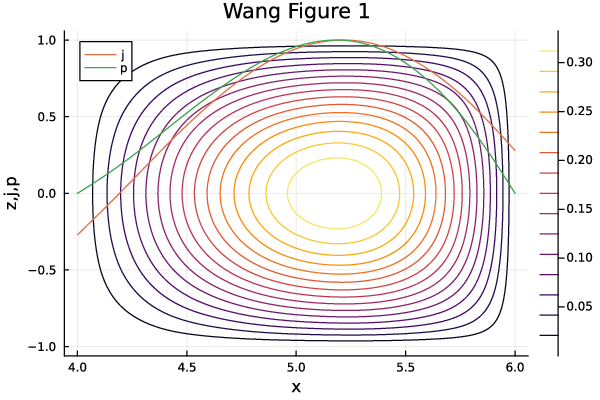
\includegraphics[scale=0.6]{imgs/c3/wang-fig-1.png}
    \caption{Figure 1 of \cite{wang-analytic-solution}. Here, the parameters are $(a_1, a_2, \alpha) = (-0.04531, -1.0808, 2.1683)$, 
    where the minor radius $a = 1$, the elongation is $k = 1$, and the major radius is taken to be $R = 5$.}
\end{figure}

\begin{figure}[h!]
    \centering
    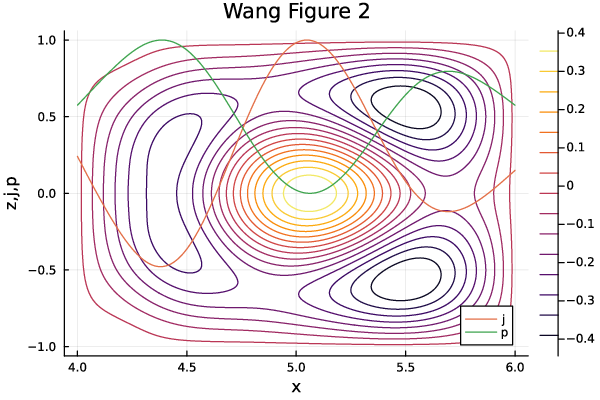
\includegraphics[scale=0.6]{imgs/c3/wang-fig-2.png}
    \caption{Figure 2 of \cite{wang-analytic-solution}. Here, the parameters are $(a_1, a_2, \alpha) = (0.01, 3.1, 5.566)$, 
    where the minor radius $a = 1$, the elongation is $k = 1$, and the major radius is taken to be $R = 5$. Note that 
    the characteristic x-point is seemingly missing from our version - this is simply an effect of Julia's plot 
    smoothing, and the data representing it is still available to us.}
\end{figure}

\begin{figure}[h!]
    \centering
    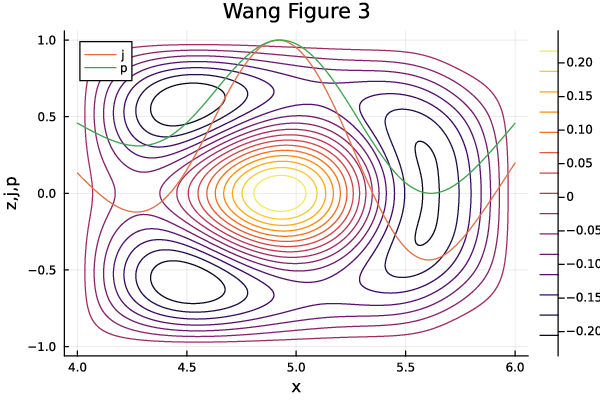
\includegraphics[scale=0.6]{imgs/c3/wang-fig-3.png}
    \caption{Figure 3 of \cite{wang-analytic-solution}. Here, the parameters are $(a_1, a_2, \alpha) = (-0.06, -0.0006, 5.50)$, 
    where the minor radius $a = 1$, the elongation is $k = 1$, and the major radius is taken to be $R = 5$.}
\end{figure}

  
\chapter{Numerical Model Fitting}
\label{chapter4}

With the ability to generate an equilibrium solution for the GSH equation from chapter \ref{chapter3}, 
our next goal is to be able 
\todo
In chapter \ref{chapter3} we developed the ability 

% 4.1.
\section{Non-Linear Optimisation}

Optimisation methods are, at their heart, minimisation problems (and dually maximisation problems, 
though the two are equivalent). We have some function $f(x)$, called the \textit{objective function},
and some domain $\Omega \subset \R^n$, and we wish to determine
$$\arg\min_{x \in \Omega} f(x)$$
Often the objective function is accompanied by a set of constraints, which more or 
less are used to define the set $\Omega$. If we let $c_i(x) \ge 0$ describe one of $k$ constraints that $f$ 
is subject to, then we can describe $\Omega$ as such:
$$\Omega := \lbrace x \in \R^n : c_1(x) \ge 0 \; \land c_2(x) \ge 0 \land \dots \land c_k(x) \ge 0 \rbrace$$

\begin{remark}
    If a given problem has no constraints (i.e. you are only presented with the task of minimising a function), then 
    this is known as an \textbf{unconstrained optimisation} problem. As soon as you add constraints however, you have a 
    \textbf{constrained optimisation} problem. Algorithms may have better or worse performance in reaching a local minimum 
    depending whether the problem is constrained or not.
\end{remark}

There are a number of difficulties that come packaged with optimisation problems. Firstly, 
the method by which you go about minimising your function is dependent on the properties of your function 
- you will have a much easier time minimising a smooth, convex function than you would a discontinuous, 
non-convex function, and different algorithms will net you varying results for each. Another factor 
that affects the choice of optimisation methods available, is the linearity of your system. Often linear systems 
can have ``nice'' methods of solving them. However, the behaviour of non-linear systems can often make them 
unwieldy when it comes to finding local and/or global minima. 

\begin{definition}[Non-linear Optimisation Problem]
    Let $x \in \Omega \subseteq \R^n$. Also let $f:\Omega \to \R$ be the objective function, and $c_i :\Omega \to \R$ and $d_j : \Omega \to \R$ be 
    constraints. Then a non-linear optimisation problem is a problem
    \begin{align*}
        &\min_{x \in \Omega} f(x) \\
        c_i(x) &\ge 0 \;\; \forall i \in \lbrace 1, \dots, m \rbrace \\
        d_j(x) &= 0 \;\; \forall j \in \lbrace 1, \dots, p \rbrace
    \end{align*}
    where one of $f$, $c_i$ and/or $d_j$ are non-linear.
\end{definition}


% 4.1.1.
\subsection{Least Squares}

Least squares problems are a subsect of optimisation problems, which are largely concerned with fitting some function to 
a set of data. Let a set of data be given $(x_i, y_i)$, where $x_i$ are independent variables, and $y_i$ are dependent variables in 
the data set. We wish to fit some function $f(x, \beta)$ to fit our data as tightly as possible, where $x$ is the independent variable 
as for the data, and $\beta$ are parameters in the function $f$ which can be varied. Let $r_i$ be the \textit{residual} error between 
a given data entry $(x_i, y_i)$ and our corresponding value for it, $f(x_i, \beta)$ for a given $\beta$. Then our goal 
(in wanting to have a function $f$ which matches the provided data) is to reduce the amount of residual error we have - to minimise it. 
We can specify this as an optimisation problem \cite{carlone-least-squares}
\begin{align*}
    \min_{\beta \in \Omega} \sum_{i = 1}^{n} \norm{r_i(\beta)}^2 = \min_{\beta \in \Omega} \sum_{i = 1}^{n} \norm{y_i - f(x_i, \beta)}^2
\end{align*}
In this case, our objective function is the equation $g(\beta) = \sum_{i = 1}^{n} \norm{y_i - f(x_i, \beta)}^2$.

\begin{remark}
    While the above norm is left general, often optimisation algorithms will take this to be the $L^2(\R^n)$ norm.
\end{remark}
\begin{remark}
    The above is, by default, an unconstrained optimisation problem. When we come to formulate our own least squares problem, we will 
    introduce our own constraints however. Additionally, the above is not specified to be linear or non-linear. In our efforts, 
    we will deal with a non-linear system.
\end{remark}

Thus, if you are provided with a set of data, and a function you wish to use to approximate the behaviour of the data, you can 
employ the use of a least squares optimisation method to manipulate that function into being as close a fit to that data as 
it can be. How we implement that optimisation is a question of algorithms, which we will now cover.

% 4.1.2.
\subsection{Optimisation Algorithms}

\begin{notn}
    When we talk about running algorithms to solve our optimisation problems, we will use a few terms. We define those here:    
    \begin{table}[h!]
        \begin{tabular}{p{3.5cm}|p{10cm}}
            \textbf{Feasible} & A problem is feasible if the algorithm is able to find an $x^* \in \Omega$ that is a local minimum and satisfies any given conditions. Otherwise, it is \textbf{infeasible}. \\ \hline
            \textbf{Objective Value} & The value of the objective function for the identified local minimum $x^* \in \Omega$, $f(x^*)$ . \\ \hline
            \textbf{ftol} & If the difference between consecutive objective function values is less than this amount, stop the optimisation algorithm and return converged \\ \hline
            \textbf{xtol} & If the difference between consecutive $x \in \Omega$ values is less than this amount, stop the optimisation algorithm and return converged \\ \hline
        \end{tabular}
    \end{table}
    
\end{notn}

The main questions that an optimisation algorithm asks at each of its iterations is: which direction should I travel, and how far 
should I travel in that direction? Algorithms that use this form of logic are called \textit{descent methods}, and a 
general approach for them is given \cite{carlone-least-squares}:

\begin{algorithm}[h!]
    \begin{algorithmic}[1]
        \State Given initial guess $x$
        \While {Convergence criteria not satisfied}
            \State Choose (unit) descent direction $\delta_x \in \R^n$
            \State Choose step size $\gamma \in \R$
            \State $\delta \leftarrow \gamma \cdot \delta_x$
            \State Update variables $x = x + \delta$
        \EndWhile
    \end{algorithmic}
\end{algorithm}
Thus, descent algorithms are distinguished by the mechanism by which they choose a descent direction, and the step size.

While the algorithms we will talk about here can be applied to optimisation problems generally, we should 
keep in mind their application to non-linear least squares problems, as this is what we will eventually deal with. 
Here we'll provide an overview of two common algorithms 
used for finding local minima of a given function. In our attempts to fit a model to some data in section 4.2, we first 
attempted to use these methods. However, due to the nature of the objective function we have, these efforts were in vain, and 
we turned to a different algorithm (MMA). Nevertheless, it is useful for intuition to see examples of other algorithms.

\subsubsection{Newton's method}
Newton's optimisation method exploits a Taylor series expansion of a given objective function. Assume that we 
want to determine $\min f(x)$, where $x,\delta \in \R^n$. We know that an expansion about $x + \delta$ is:
\begin{equation*}
    f(x+\delta) \approx h(x+\delta) := f(x) + \nabla f(x)^{T} \delta + \frac{1}{2}(\delta)^{T} \nabla^2 f(t) \delta
\end{equation*}
where $\nabla^2$ denotes the Hessian. We want to find a turning point (minimum) of the above, so we can simply set its 
derivative to be $0$. This gives us
\begin{equation*}
    \nabla f(x) + \nabla^2 f(x) \delta = 0
\end{equation*}
This tells us that the optimal descent direction (and step size) is
\begin{equation*}
    \delta = - \gamma \left [  (\nabla^2 f(x))^{-1} (\nabla f(x)) \right ]
\end{equation*}
where $0 < \gamma \le 1$ is a chosen step size, which can be tailored to a given problem. 

\begin{remark}
    As Newton's method only necessitates that the objective function be twice differentiable, it is applicable to 
    optimisation problems generally (i.e. it is not restricted to constrained nor unconstrained problems, nor does it differentiate 
    between linear and non-linear problems).
\end{remark}

\subsubsection{Gradient descent}
Gradient descent is an approach which has strong intuitive roots. If you were at the top of a hill, and wanted to get 
to the bottom as fast as possible, then you might choose to go down the steepest point you see around you. This is 
essentially what gradient descent does. For an objective function $f(x)$, assuming that it is differentiable 
for some neighbourhood of a point $a \in \R^n$, then the optimal descent direction is $- \nabla f(a)$. This can, 
similar to Newton's method, be scaled by a step size $\gamma$ to slow / speed up this process, though the value of 
this is dependent on the optimisation problem you're investigating (note that, similar to Newton's method, 
the gradient descent method can be applied to a large class of problems).

\subsubsection{MMA}
One of the problems we encountered in our data fitting attempts (which we will see in the next section), is that 
of asymptotic behaviour which affects convergence of our algorithms. Thus, we sought to employ the use of an algorithm 
which was more resistant to such behaviour in an objective function. This led to the discovery of the Method of Moving 
Asymptotes algorithm, developed 
by Svanberg \cite{mma}. While its implementation details are a bit volumous to repeat here, in essence, it works by creating 
convex sub-problems around potential local minima, and attempts to minimise these individually. It repeats this process until 
it is no longer decreasing, and returns the most recent potential local minima it found. This algorithm is 
useful to us two main reasons: 1. it is still as robust an optimisation method as Newton's method and gradient descent, in that it 
can handle a host of optimisation problems (including non-linear problems); and 2, it is more resistant to the asymptotic behaviour.

In our code we use an implementation provided by the NLopt package, a nonlinear optimisation library for Julia \cite{nlopt}. The NLopt
library, in iniitialising an optimisation problem for MMA, requires information about the objective function, its partial derivatives, 
and any constraints, if they exist (which they will for us, but we'll note on that shortly). Thus, when it comes to constructing 
our system, we must provide the objective function naturally, but also its partial derivatives with respect to our paramters.

% 4.2.
\section{GSH Parameter Fitting}

In the previous chapter we were able to, given $P := (a_1, a_2, \alpha)$, reproduce results from Wang, including 
the poloidal magnetic flux, current density profile, and pressure density profile. However, in reality, we will 
not know these parameters $P$ for a given system - yet we are entirely dependent on them for describing our system. 
We then face a problem, which is that if we wish to vary our system, or if we wish to describe a real tokamak's dynamics,
we need some way to determine what $P$ should represent the system we're investigating. 

Looking forward a bit, we know that from the ISTTOK project we have time series current density profile and pressure density profile data 
available to us. Thus we may wish to utilise at least one of these in determining $P$ - and this is exactly what we will do. 
In the previous section we built the theory for, given a set of data, fitting a function $f$ with variables $\beta$ which can be varied, 
which is exactly the challenge we now face. 

We could seek to use both the current density profile and pressure density profile, and could build an objective function around this. However, 
we will also note that we wish to verify our results - as such, it may be prudent to leave one of these data sets available for comparison instead. 
With a bit of prescient knowledge we may realise that derivatives are much easier to calculate for the current density profile, and so choose 
to build our objective function around this, reserving pressure density data for comparisons instead. In the spirit of laziness, this is 
exactly what we do.

In this chapter we will not concern ourselves with experimental data however - that is the task of chapter \ref{chapter5}. Here we 
will work with contrived data. With our ability to specify parameters $P$ and derive the equilibrium solution from that, we can generate 
our own simulated current density profile data, and then attempt to work in the opposite direction - to fit parameters $P'$ to that data, 
which we can then compare to $P$ for accuracy.

% 4.2.1
\subsection{Optimisation Problem}

\subsubsection{Objective Function}
Let $(x_i, d_i)$ denote a data entry for the current density profile. We will perform a least squares optimisation, and so need to specify $f(x, \beta)$. 
In our case, $\beta = P = (a_1, a_2, \alpha) \in \R^3$, and
\begin{equation*}
    f(x, \beta) = j_{\phi}(x, z) = -a_1 x + \frac{1}{x} a_2 + \frac{\alpha^2}{x} \psi(x, z)
\end{equation*}
Note here though that the current density profile is taken to be for $z = 0$. Additionally, we can transform our current density profile function 
$\vec{j}_{\phi}$ to also be in terms of $P$ by specifying them as independent variables, and so the above is more accurately stated
\begin{equation*}
    f(x, \beta) = j_{\phi}(x, P) = -a_1 x + \frac{1}{x} a_2 + \frac{\alpha^2}{x} \psi(x, 0, P)
\end{equation*}
Assume that we have $N$ data entries for the current density profile available to us. Then, our least squares optimisation problem is given:
\begin{align*}
    \notag& \min_{\beta \in \Omega} \sum_{i = 1}^{N} \norm{d_i - f(x_i, \beta)}^2 \\
    \iff& \min_{P \in \Omega} \sum_{i = 1}^{N} \norm{d_i - j_{\phi}(x, P)}^2 
\end{align*}
for now we will take $\Omega = \R^3$, however this will change shortly. This, however, is the objective function we seek to minimise - 
in the hopes that the resulting parameter $P$ will let $j_{\phi}(P)$ accurately describe the current density profile we expect, and thus 
the rest of the system will follow suit.

\subsubsection{Partials}
We require $\nabla g(P)$, where $g(P) = \sum_{i = 1}^{N} \norm{d_i - j_{\phi}(x, P)}^2$. We'll calculate each individually:
\begin{align*}
    \pdv{g(P)}{a_1} &= \pdv{a_1} \sum_{i = 1}^{N} \norm{d_i - j_{\phi}(x, P)}^2 \\
    &= \pdv{a_1} \sum_{i = 1}^{N} \left ( d_i - j_{\phi}(x, P) \right )^2 \\
    &= 2 \sum_{i=1}^{N} \left ( \pdv{a_1} (d_i - j_{\phi}(x, P)) \right ) \\
    &= -2 \sum_{i=1}^{N} \left ( d_i - \pdv{a_1} j_{\phi}(x, P) \right ) j_{\phi}(x, P)
\end{align*}
By similar calculation, we get the partials for $a_2$ and $\alpha$ to be:
\begin{align*}
    \pdv{g(P)}{a_2} &= -2 \sum_{i=1}^{N} \left ( d_i - \pdv{a_2} j_{\phi}(x, P) \right ) j_{\phi}(x, P) \\
    \pdv{g(P)}{\alpha} &= -2 \sum_{i=1}^{N} \left ( d_i - \pdv{\alpha} j_{\phi}(x, P) \right ) j_{\phi}(x, P)
\end{align*}
Thus, we now only need the partials of the toroidal current density with respect to each element of $P$, which we provide below
\begin{align*}
    \pdv{j_{\phi}(x, P)}{a_1} &= \pdv{a_1} \left ( -a_1 x + \frac{1}{x} a_2 + \frac{\alpha^2}{x} \psi(x, z, P) \right ) \\
    &= -x + \pdv{a_1} \left ( \frac{\alpha^2}{x} \psi(x,z, P) \right ) \\
    &= -x + \alpha^2 \sum_{n = 1}^{M} \sum_{l = 0}^{M-1} \frac{2(-1)^l [c_n J_1(\mu_n x) + N_1(\mu_n x)]}{k v_l a_n^d (\alpha^2 - \lambda_{n,l}^2)} \left [ \frac{1}{\mu_n} x'^2 \left (c_n J_2(\mu_n x') + N_2(\mu_n x') \right ) \right ]_{R_0 - a}^{R_0 + a} \\
    \pdv{j_{\phi}(x,P)}{a_2} &= \frac{1}{x} + \alpha^2 \sum_{n = 1}^{M} \sum_{l = 0}^{M-1}  \frac{2(-1)^l [c_n J_1(\mu_n x) + N_1(\mu_n x)]}{k v_l a_n^d (\alpha^2 - \lambda_{n,l}^2)} \left [ \frac{1}{\mu_n} \left ( c_n J_0(\mu_n x') + N_0(\mu_n x') \right ) \right ]_{R_0 - a}^{R_0 + a} \\
    \pdv{j_{\phi}(x,P)}{\alpha} &= \frac{2\alpha}{x} \psi(x, 0, P) + \alpha^3 \sum_{n=1}^{M} \sum_{l=0}^{M-1} \frac{4(-1)^l a_n^u}{k v_l a_n^d (\alpha^2 - \lambda_{n,l}^2)} \left [ c_n J_1(\mu_n x) + N_1(\mu_n x) \right ]
\end{align*}
With these, we have the partial derivatives (with respect to our parameters) of our objective function, and we have our objective function. 
Additionally, we have our data (emulated current density profile data, which we generated from the prescribed $(a_1, a_2, \alpha)$ values 
in Wang \cite{wang-analytic-solution}). This is everything required by NLopt for performing an optimisation, and so the only thing left to do is optimise, and see our results!


% 4.2.2
\subsection{Parameter Space}

Initially, our efforts in fitting a set of parameters to a given input of current density profile data were without accomplishment, as the 
optimisation methods failed to converge (reaching max iteration counts before reaching an acceptable objective value). Given we have 
omnipotent knowledge as to what our $P = (a_1, a_2, \alpha)$ values should be, we can look at the parameter space around 
these values to see why our optimisation algorithm might be falling over. The results are telling, and can be seen in figures \ref{heat-1-entire} 
to \ref{heat-3-entire}


\begin{figure}[h!]
    \centering
    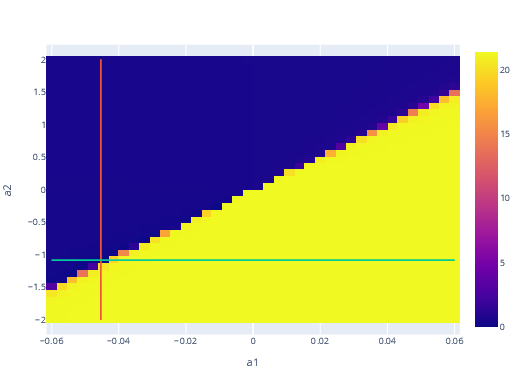
\includegraphics[scale=0.7]{imgs/c4/heat-1-entire.png}
    \caption{Objective value heatmap for fixed $\alpha$, with varying 
    $a_1$ and $a_2$}
    \label{heat-1-entire}
\end{figure}

\begin{figure}[h!]
    \centering
    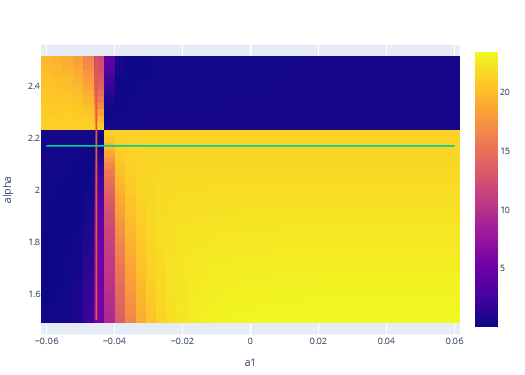
\includegraphics[scale=0.7]{imgs/c4/heat-2-entire.png}
    \caption{Objective value heatmap for fixed $a_2$, with varying 
    $a_1$ and $\alpha$}
    \label{heat-2-entire}
\end{figure}

\begin{figure}[h!]
    \centering
    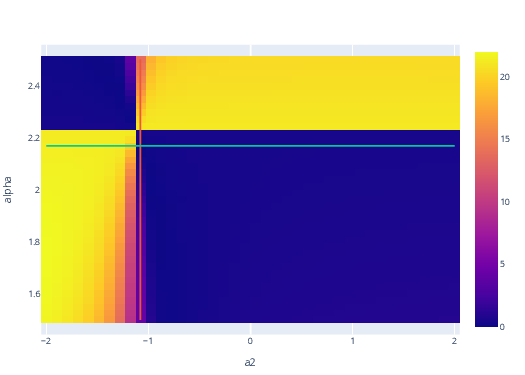
\includegraphics[scale=0.7]{imgs/c4/heat-3-entire.png}
    \caption{Objective value heatmap for fixed $a_1$, with varying 
    $a_2$ and $\alpha$}
    \label{heat-3-entire}
\end{figure}\newpage
The lines here point to the expected $(a_1, a_2, \alpha)$ values, and for each one 
we fix the parameter not being varied to be its expected value. Nevertheless, as we can see, our 
parameter space is quite binary, in that the distinction between suitable parameters and not is quite sharp, 
but with plateau's on either side - a nightmare situation for optimisation algorithms. If we zoom in 
around our expected parameters we indeed see even more strongly the sensitivity of our objective value to fluctuations in 
input parameters - see figures \ref{heat-1-zoomed} to \ref{heat-3-zoomed} in Appendix A.

Some of this behaviour is the result of the $(\alpha^2 - \lambda_{n,l}^2)^{-1}$ term introduced 
by $\psi$ in our objective function - it is this which motivates our usage of the MMA optimisation 
algorithm over more traditional methods like gradient descent, as we discussed in the previous section. 
However, as it stands - as an unconstrained optimisation problem - this is clearly still insufficient. 
One initial thought might be that our problem is simply underdetermined, and that by introducing more 
data we may improve the ability of our model to converge. However, as we see in figures \ref{heat-1-both} to \ref{heat-3-both},
the inclusion of pressure density profile data in our fitting attempts does not vastly improve our parameter space.

As such, the inclusion of extra data does not seem promising in our efforts to find a suitable set of parameters. Instead, 
our next effort was to constraint our problem - given we know what to expect our $P = (a_1, a_2, \alpha)$ values 
to be, we can constrain our parameter space by specifying a small offset for each. For example, 
if we know our parameter set is supposed to be $P' = (a_1', a_2', \alpha')$, then we can set
$$\Omega = [a_1' - \epsilon_{a_1}, a_1' + \epsilon_{a_1}] \times [a_2' - \epsilon_{a_2}, a_2' + \epsilon_{a_2}] \times [\alpha' - \epsilon_{\alpha}, \alpha' + \epsilon_{\alpha}]$$
For our intial parameter guess $P_0$ we can pick some random element of $\Omega$. When we introduce these constraints 
and turn our problem into a constrained optimisation problem we see significantly improved 
results, and our model converges - see figure \ref{solved-fig-1} as a recreation of figure 1 from Wang 
using simulateed current density profile data.

\begin{figure}[h!]
    \centering
    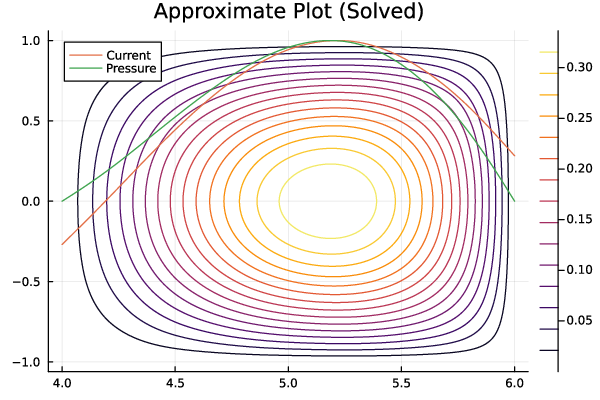
\includegraphics[scale=0.8]{imgs/c4/solved-fig-1.png}
    \caption{Equilibrium solution for the parameter set $P$ that we determine via optimisation, starting with a 
    set of current density profile data. This matches the expected figure 1 from Wang \cite{wang-analytic-solution}.}
    \label{solved-fig-1}
\end{figure}

\begin{figure}[h!]
    \centering
    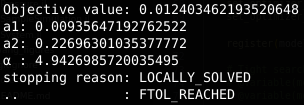
\includegraphics[scale=1]{imgs/c4/converged.png}
    \caption{Text output of our code showing convergence of our model.}
\end{figure}

Now that we can, for a given set of data, accurately derive the associated equilibrium solution, 
our next goal is simulate a current inversion given said data.

% 4.3
\section{Simulated Current Reversals}

We have the ability to solve for $P = (a_1, a_2, \alpha)$, and so now we will draw upon our 
work in chapter \ref{chapter3} in perturbing our equilibrium solution to simulate the effects of 
a time evolution, and in doing so, will observe how the system reacts.


% 4.3.1
\subsection{Method of Reversal}


\red{Linearly vary current. Could talk about alternatives - i.e. if 
our time perturbation had not been linear but had been trigonometric (to 
fit with a larger scope AC simulation) then our current reversal method 
here could be different}

\red{Feed solved parameters into guess for next. Emphasise problem of not knowing 
the initial ones nonetheless}


% 4.3.2
\subsection{Results and Explanations}

\red{Have still frame shots of the result of that (3x3 tiles?)}

\red{Show the slow version, then the 'zoomed' in version}

\red{Highlight magnetic field topology breaking - suggests RE population generation}

\red{Comment on feasibility of the behaviour - e.g.pressure density profile follows 
magnetic field axis, but then there are things like current densities 
at the edge of the reactor}


  
\chapter{Comparison with Experiment}
\label{chapter5}

% 5.1.
\section{ISTTOK}

The ISTTOK project is a reactor based in Lisbon, Portugal, used for plasma science research by the 
University of Lisbon. It is this reactor which found 
no evidence for the existence of anti-parallel currents in the ramp down phase, contradicting 
the hypothesis put forward to explain the presence of a residual plasma during the quiescent 
current cycle, as we discussed in the introduction \cite{malaquias-matthew}. 
This hypothesis was initially supported by data from from the CT-6B Tokamak by Huang et. al \cite{huang-ct-tokamak} however, 
and so no consensus exists on whether these currents exist, and what the cause of the runaway electrons is in cases of 
AC Tokamak ramp downs. In this chapter we attempt to use our model to describe the current density profile, pressure density profile, 
and poloidal magnetic field topology, given some data provided by ISTTOK.


% 5.1.1
\subsection{Heavy Ion Beam Diagnostics}

The data we have available to us is time slices of current density profile, pressure density profile, 
and $v_{\text{loop}}$ data for the ramp down phase of a run of the ISTTOK reactor. Before 
we ``plug and play'' with this data though, it's important to understand where it has come from. 

One of the flagship features of the ISTTOK reactor is its heavy ion beam probe, which enables 
the measurement of the plasma temperature, electron density, and plasma potential ($v_{\text{loop}}$) 
data. Theoretically it is able to produce a one dimensional profile of each of these components - these 
can then be used to infer the value of other plasma properties, such as the current density profile \cite{ion-beam-diagnostics}.

We will stave off delving too deep into the physics here, and will instead seek to provide an intuition for 
the functioning of the beam. A heavy ion beam is a measurement tool that works by injecting heavy charged 
particles (ions) into a charged medium, at speed. The charged medium in our case is the plasma. For a Tokamak, 
a beam of positively charged ions (specifically, atoms with one extra electron) are injected into the plasma, 
known as the ``primary beam'', and commonly consists of one of $\text{Cs}^{+}, \text{Rb}^{+}$. These 
ions are injected perpendicular to the toroidal magnetic field (that is to say, in line with the poloidal 
magnetic field). The idea behind this is that these positively charged atoms ($I^{+}$) will interact with the negatively charged 
electrons in our plasma in a way that we can measure, which will provide us insight into the properties 
of electron populations in our plasma. When $I^{+}$ interacts (collides) with an electron in the plasma, 
it is likely to become ionised further, becoming $I^{2+}$. The property in our plasma that we then 
exploit to measure this change is the Lorentz force, which, to recall, states 
$$\vec{F} = q(\vec{E} + \vec{u} \times \vec{B})$$
where, crucially, $q$ represents a particle's charge as it moves through an magnetic field $B$ with velocity $\vec{u}$, and an electric field $E$ present. 
From this we can infer that the forces acting on a particle will increase as the charge 
increases. The effects of this increased ionisation of our heavy ions thus increases their Larmor radius
(oscillatory movement of charged particles in a magnetic field) relative to their single-ionised counterparts, 
which changes their trajectory in the plasma. In our Tokamak we then position a charged particle detector on the opposite 
side of our heavy ion beam's injection point, which we use to measure distributions of received charged 
particles. Form this we can infer information about the presence of negatively charged particles 
(predominantly electrons) in the $1D$ profile that our primary beam follows by measuring the 
quantity of charged particles detected at different positions on our detector. Ingenious! A graphic depicting this 
is given in figure \ref{heavy-ion-beam}.

\begin{figure}[h!]
    \centering
    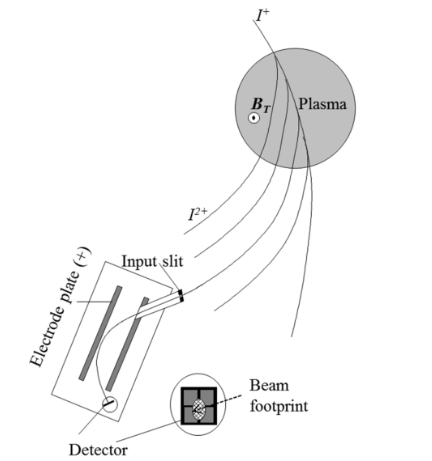
\includegraphics[scale=0.8]{imgs/c5/ion-diagnostics.png}
    \caption{Simplified depiction of an ion beam's injected ions having their trajectories manipulated by the plasma they travel through, and how that is 
    subsequently detected. Diagram taken from \cite{ion-beam-diagnostics}.}
    \label{heavy-ion-beam}
\end{figure}

While here we've provided what is hopefully an intuitive understanding for how a heavy ion beam is utilised for data 
collection in a Tokamak, we have skipped much of the nitty-gritty details for actual data derivation. Most importantly for us to note
however, is that ISTTOK does not directly measure the current or pressure density profiles, but instead 
infers this data from poloidal magnetic field profile information afforded to us by the heavy ion beam. 
As one might expect, there is a large margin for 
error introduced in these measurements (and subsequent calculations) when doing so. Quoted unofficially, we can expect errors in 
current density profile data to be up to an order of $\pm30\%$. While we don't have access to the explicit uncertainty in our data, we can keep this in mind when 
fitting our parameters $(a_1, a_2, \alpha)$ to the ISTTOK data, and justify some decisions we make further down.

% 5.1.2
\subsection{Reactor Specification and Data}

\noindent\textbf{Reactor Specification}\\
The ISTTOK reactor specification is given below:

\begin{table}[h!]
    \centering
    \begin{tabular}{|c|c|}
    \hline
    Property           & Value                                                 \\ \hline
    Major Radius ($a$)       & $0.46\text{m}$                                                 \\ \hline
    Minor Radius ($R_0$)      & $0.085\text{m}$                                              \\ \hline
    Plasma Current ($I_p$)   & $~4-6\text{kA}$ \\ \hline
    \end{tabular}
    \caption{Relevant ISTTOK reactor parameters \cite{malaquias-matthew}}
\end{table}

Of particular emphasis, this configuration satisfies the requirement for a large aspect Tokamak as required for 
our Grad-Shafranov-Helmholtz model, with $A = R / a = 5.4 \gg 1$.

\noindent\textbf{Available Data}\\
\noindent
The data we have is for a series of 20 time slices from $30.53\text{ms} - 31.93\text{ms}$ of 
a run of ISTTOK. Of interest, the average confinement time for a plasma in ISTTOK is approximately
$0.4\text{ms}$ \cite{malaquias-matthew}. For each of these time slices there are $18$ 
measurements at uniformly distributed discrete intervals across the cross section of the reactor; 
for $x \in [-8.5\text{cm}, 8.5\text{cm}]$ and $z = 0$. For this domain we have data for the 
current density profile, and the pressure density profile. From this data, we additionally have inferred $I_p$ and $V_{\text{loop}}$ data for each time slice.

In our simulations we will use the current density profile data to fit our parameters $(a_1, a_2, \alpha)$. 
In the work that we did we did not initially seek to additionally use the pressure density profile data in fitting 
these paramters for two reason:
\begin{enumerate}
    \item We wish to have some data to compare our results to. From the $(a_1, a_2, \alpha)$ we get from our 
    minimisation algorithm we can calculate a pressure density profile and compare it to the experimental data for accuracy
    \item In our simulations we explored the case of having limited current density profile data and attempting to 
    fit parameters to that, and found that we were able to deterine parameters sufficiently accurate to represent the system.
\end{enumerate}
While we will make comparisons with the pressure density profile data, another avenue we could 
have explored was to incorporate the pressure density profile into the data fitting. Initial testing with this did not improve convergence of the optimisation algorithm for those cases in 
which it struggled, however our testing was also not exhaustive in this manner, and the inclusion of this 
data combined with some changes in the approach to fitting our model to the data, could well result 
in a more accurate result. Ideas for further work around this are discussed in chapter \ref{chapter6}.

A representative time slice is provided in figure \ref{current-profile-unnormalised-0}

\begin{figure}[h!]
    \centering
    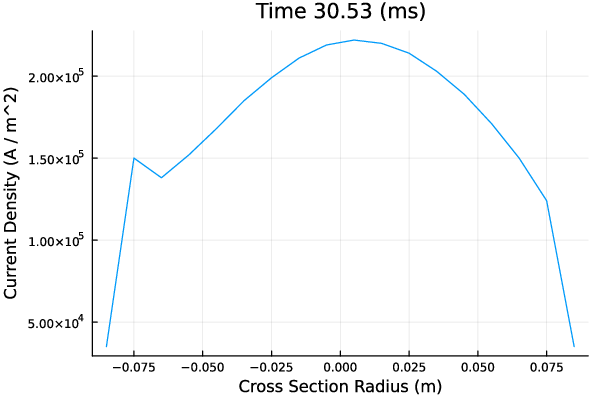
\includegraphics[scale=0.6]{imgs/c5/current-profile-unnormalised-0.png}
    \caption{Current density profile for the beginning of a ramp down in ISTTOK. The cross section radius is centred 
    with respect to the major radius.}
    \label{current-profile-unnormalised-0}
\end{figure}\newpage

The $I_p$ time evolution is also provided for reference in figure \ref{ip-time}. This showcases how the plasma's current 
changes during the ramp down phase.
\begin{figure}[h!]
    \centering
    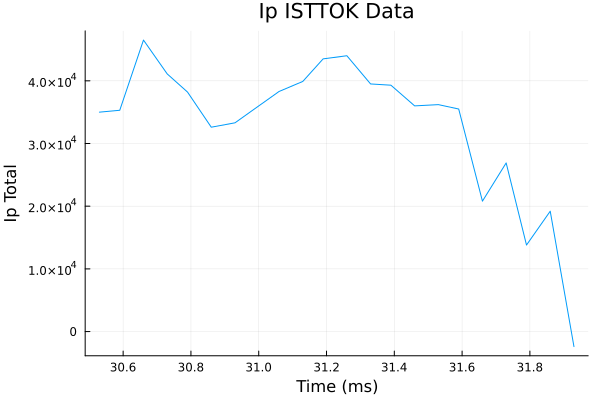
\includegraphics[scale=0.6]{imgs/c5/ip_time_data.png}
    \caption{Plasma current ($I_p$) during the ramp down phase of a run of the ISTTOK reactor in AC operating mode.}
    \label{ip-time}
\end{figure}\newpage

% 5.2
\section{Parameter Fitting}

\subsection{Results}

\subsubsection{Initial Attempts}
We use the same process as we did when initially fitting the parameters $(a_1, a_2, \alpha)$ to data, though instead of contrived 
current inversion data we of course use the data we have from ISTTOK here. Our initial results 
showed a resistance of our model to fitting to the data, as can be seen by the poor fit for 
the current density profile in figure \ref{comparison-current-0-unfiltered}. All of our results are available in the source code under 
under the ``experiments/isttok/current\_solving\_comparison/graphs/'' directory \cite{project-source}.
Here we will highlight a couple representative examples, but will discuss the general trend 
of all our results.

\begin{figure}[h!]
    \centering
    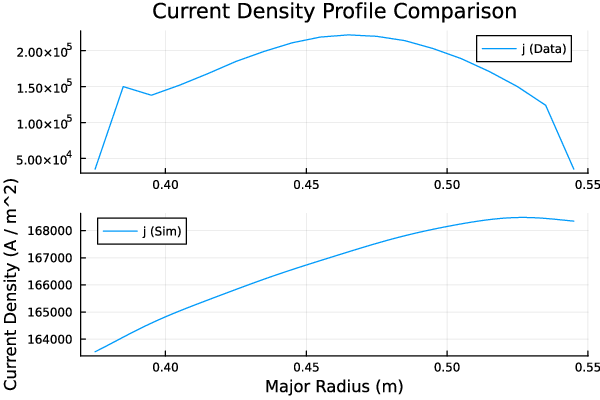
\includegraphics[scale=0.7]{imgs/c5/comparison-current-0-unfiltered.png}
    \caption{ISTTOK current density profile contrasted with our simulated current density profile
    after fitting against the former in order to derive $(a_1, a_2, \alpha)$. This is the first 
    time slice, i.e. at the start of the ramp down.}
    \label{comparison-current-0-unfiltered}
\end{figure}
Purely by visual inspection we can see this is not a close fit, 
however this discrepancy becomes more pronounced as we progress through the remainder of our time slices. 
This effect can be seen in figure \ref{comparison-current-15-unfiltered}, where our simulation is 
even more considerably differentiated from the data.

\begin{figure}[h!]
    \centering
    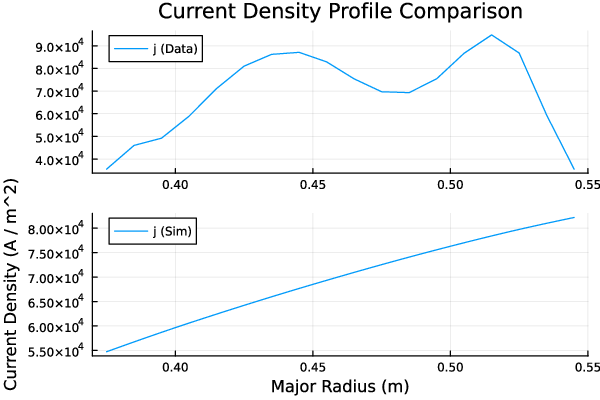
\includegraphics[scale=0.7]{imgs/c5/comparison-current-15-unfiltered.png}
    \caption{ISTTOK current density profile contrasted with our simulated current density profile
    after fitting against the former in order to derive $(a_1, a_2, \alpha)$. This is the 15th 
    time slice, i.e. approximately half way through the transition.}
    \label{comparison-current-15-unfiltered}
\end{figure}

Here we begin to see a current hole develop at (what we for now presume, but will later 
observe) the position of the on-axis magnetic island. This is an important feature to be 
able to characterise in our simulations, however is clearly missed in our simulated current. In fact, 
it seems that the general features of our simulated current density profile remain largely unchanged 
from our initial results - we will comment on why this is so in a minute.

We can also (for completeness here) compare the last time slice, which is the first and only 
data entry we have showing the start of the ramp up phase, or in other words, the period immediately 
proceeding the conclusion of the ramp down phase we are investigating. This comparison is shown 
in figure \ref{comparison-current-20-unfiltered}.
\begin{figure}[h!]
    \centering
    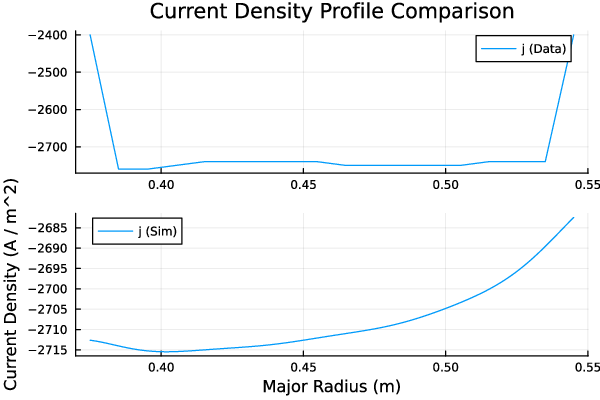
\includegraphics[scale=0.7]{imgs/c5/comparison-current-20-unfiltered.png}
    \caption{ISTTOK current density profile contrasted with our simulated current density profile
    after fitting against the former in order to derive $(a_1, a_2, \alpha)$. This is the last 
    time series data entry we have, and is after the ramp down phase has concluded / the 
    start of the next cycle's ramp up phase.}
    \label{comparison-current-20-unfiltered}
\end{figure}\newpage

Recall that, while the initial parameter guess is currently hand picked (with note on 
alternatives proposed in chapter \ref{chapter6}), parameter guesses for subsequent iterations of our 
simulation are informed by the previously solved-for parameters. This means any initial error in choice of parameters 
will be detrimental to all following simulations.

We can see the effects of this more prominently by also observing the change in magnetic field toplogy 
as the current and pressure data vary. Or rather, we should say, the lack thereof. Figures \ref{mag-field-0} - \ref{mag-field-20}
show the poloidal magnetic field topology for the representative time slices we've picked. Note again that results for all 
time slices can be found in the open sourced GitHub repository in \cite{project-source}.

\begin{figure}[h!]
    \centering
    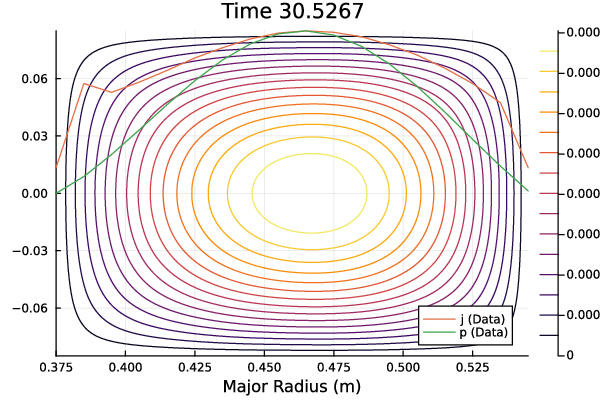
\includegraphics[scale=0.7]{imgs/c5/magnetic-field-0.png}
    \caption{Poloidal magnetic field (simulated) for a given $(a_1, a_2, \alpha)$ parameter set which is derived 
    from the current density profile data present in the graph. The pressure profile is similarly given. Both current 
    and pressure density profiles are normalised.}
    \label{mag-field-0}
\end{figure}\newpage

\begin{figure}[h!]
    \centering
    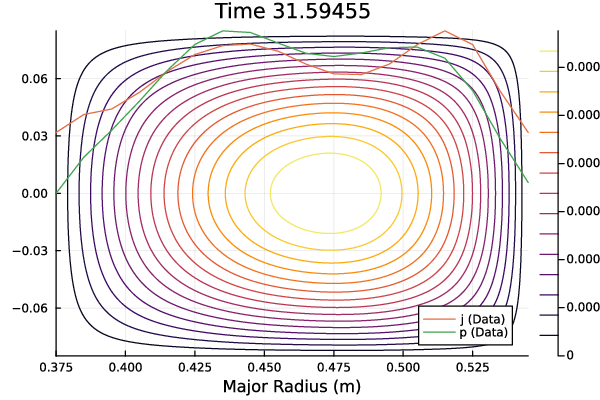
\includegraphics[scale=0.55]{imgs/c5/magnetic-field-15.png}
    \caption{Poloidal magnetic field (simulated) for a given $(a_1, a_2, \alpha)$ parameter set which is derived 
    from the current density profile data present in the graph. The pressure profile is similarly given. Both current 
    and pressure density profiles are normalised.}
    \label{mag-field-15}
\end{figure}

\begin{figure}[h!]
    \centering
    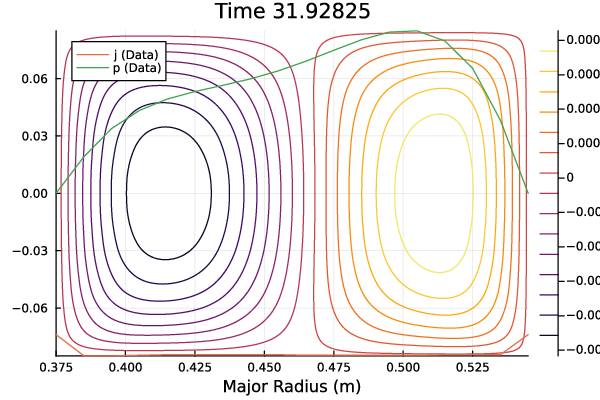
\includegraphics[scale=0.55]{imgs/c5/magnetic-field-20.png}
    \caption{Poloidal magnetic field (simulated) for a given $(a_1, a_2, \alpha)$ parameter set which is derived 
    from the current density profile data present in the graph. The pressure profile is similarly given. Both current 
    and pressure density profiles are normalised.}
    \label{mag-field-20}
\end{figure}\newpage
We find there is minimal variation in magnetic field line toplogy between all the time slices, with exception 
of the last slice, which sees a drastic change. There is a slight drift tendency towards the external wall of the reactor (rightwards in our graphs), 
which might suggest some Shafranov shift of the plasma - though, given the misrepresentative nature of the simulated 
magnetic field lines generally, it is unlikely this is an actual result. We can further support the argument that 
this is not an accurate magnetic field topology as time progresses, as the pressure density profile in 
figure \ref{mag-field-15} suggests the formation of two distinct, or at least a partially split single, plasma, with two 
distinct current densities (i.e., that there are at least two magnetic islands present). However, the simulated magnetic field (which remains largely unchanged from the 
initial simulation iteration) suggests only the existence of a single magnetic island. We should note though, that 
figure \ref{mag-field-0} shows a magnetic field line toplogy which is consistent with where the data suggests the primary 
plasma density should be - this being despite a seemingly large discrepancy between our simulated current density and the 
provided data. Nevertheless, the result is clear - the simulation, in this form, is insufficient in modelling accurately the behaviour of the 
plasma, at least with respect to what is expected from the data we have available.

Our initial efforts seem fleeting in their attempt to accurately model the system. However, that does not mean that 
our efforts should stop there. Whereas previously we politely 
requested any mathematicians avert their gaze at the crimes we were committing, it is only 
fair that we also at some point request any scientists to turn a blind eye to the 
crimes we will momentarily commit. This is that point. 
In the previous section we noted that there is a considerable uncertainty accompanying our data
(see, for instance, figure \ref{ip-time}, which intuitively we expect to be a smooth function of radial distance, 
yet is quite nonsmooth). We thus have some (limited) agency to manipulate our data to be more aligned 
with what we would expect.


\subsubsection{Data Cleanup and Second Attempt}
With the note that our data has considerably uncertainty in it, and considering the 
relatively few data entries we have, we might make some observations about the data 
we do have available, and the general physical properties we would expect it to exhibit 
with relation to the other data points we have available.

First, we'll note the (accusedly) extraneous data entries in the first time slice. Refer again 
to figure \ref{current-profile-unnormalised-0}. There are two irregularities we can note:
\begin{itemize}
    \item There is a sharp increase in current density at the $-0.065\text{m}$ offset. Physically, unless 
    there was anomalous behaviour inside the reactor, we would not expect this measurement, while the general 
    behaviour of the rest of the profile relative to this entry is consistent with a plasma density being confined to 
    the magnetic axis within the reactor. Thus, we can (to test) make an assumption that this entry is a result of imprecision in 
    the data collection, and remove it from our fitting data.
    \item At the bounds of the reactor the current density decreases significantly faster than the general trend of the 
    rest of the data. Physically this is consistent with what we would expect - that as we approach the edge of our reactor there is 
    less plasma density and less current. However, we also know our analytic current density profile to be $C^{2}$ continuous, 
    and such sharp jumps will affect our ability to fit to this data. Thus by removing this information we can potentially 
    increase the performance of our data fitting.
\end{itemize}
We see the resulting current density profile in figure \ref{comparison-current-0-edited}. It is clear that the general behaviour 
of our current density profile is more consistent with that of the data now. We can observe that the magnitude of the densities is 
still, however, quite distinct. There are a couple considerations we could make here. First is that, this is evidence that 
our model is not fitting to the data as closely as we'd like yet, and so extra work can be done to attempt to improve this. 
The second would be that, while the scale of the current density is inconsistent with the data, it may be that we can still sufficiently 
make statements about the generation of runaway electron populations, and so it perhaps is (for our intended purposes) irrelevant 
whether the scale is precise or not. More important to us is the topology of the poloidal magnetic field, which in our model is 
informed more by the radial positioning of current density masses than the strength of those densities (as we highlighted in our 
simulations section). We can see in figure \ref{mag-field-edited-data-0} that the magnetic field topology for the manually edited data 
is consistent with where the pressure and current density profiles suggest the primary magnetic island should be. Additionally, it 
appears this is more in agreement than the pre-processed data, as the positioning of the primary magnetic island is more 
accurate to what we expect than we observed in figure \ref{mag-field-0}.

\begin{figure}[h!]
    \centering
    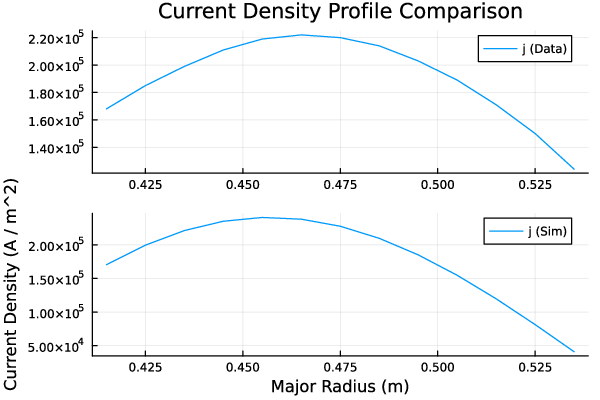
\includegraphics[scale=0.65]{imgs/c5/comparison-current-edited-0.png}
    \caption{Comparison of simulated and data current density profiles, after we rid the data of potentially eroneous data entries.}
    \label{comparison-current-0-edited}
\end{figure}
\begin{figure}[h!]
    \centering
    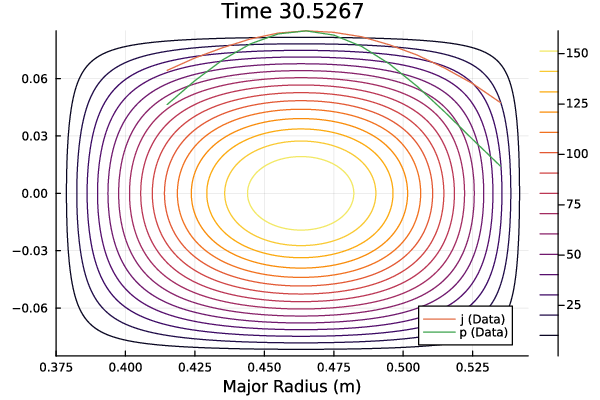
\includegraphics[scale=0.65]{imgs/c5/mag-field-edited-data-0.png}
    \caption{Simulated magnetic field topology for the stripped data. Current and pressure density profiles given are normalised, 
    and provided by the data.}
    \label{mag-field-edited-data-0}
\end{figure}\newpage

These (albeit preliminary) results would seem to suggest that, after some ``cleaning'' of the data, our model is able to 
produce results that are at least consistent with how we would expect our system to behave given the data. 

Nevertheless we face another problem which, as of writing, remains unresolved. While we are able to clean our data 
for the first time slice as what we deemed ``erroneous'' data entries were easy to identify, this is not the case for the majority 
of the remaining data we have. This is partly a problem of labour, more problematic is the that of correctly determining which 
data points to classify as erroneous - if any can even be deemed so.



\subsubsection{Alternative Data Coddling Methods and Steps Forward}
Here we have simply removed potentially erroneous data points from our set, and continued on as if they never existed. 
However, especially as we don't have access to a great many discrete measurements, this is not an ideal situation. 
There are alternative approaches to post-processing the data that could be used, and comparisons made to deem which is 
most suitable for our data fitting purposes. For example, it could be prudent to, after removing these erroneous data points, 
perform an interpolation using the remaining points. This would have the benefit of providing a data set with data that was 1. 
more volumous, and 2. smoother.

We could also interpolate in another dimension - time. One potential explanation for the difficulty our model has in moving between 
time slices in the data is that the time variation between them is too large with respect to the time perturbation expansion we performed 
in chapter \ref{chapter3}. As such, we could take two consecutive time slices of data and linearly interpolate them, introducing 
many more time slices in between. This would restrict our parameter space further, improving our optimisation, and, combined with 
the previous point about interpolating between data points, could see an improvement on the accuracy of our model.

Additionally, we face the issue that the simulation is very sensitive to the initial parameters chosen. This is directly related 
to the parameter space issue we identified in the chapter \ref{chapter4}, which is that discontinuities introduced by the $\alpha$ 
parameter lead to a high false positive rate. For the above simulations we have achieved some 
results by hand picking an initial parameter guess via manual inspection of the parameter space - this, however, is obviously insufficient 
for more general simulations. A potential resolution for this is proposed in the next chapter, and is the subject of ongoing work.
  
\chapter{Blue Skies and Horizons}
\label{chapter6}

% 6.1
\section{Conclusions}

In this thesis we've built up an ability to reason about perturbations in time about 
equilibrium solutions to a variant of the Grad-Shafranov Equation. We did this with the intent 
of modelling the ISTTOK reactor's ramp down phase as a tool for identifying 
causal mechanisms for the generation of runaway electrons. Our model, using current 
density profile data provided by the ISTTOK project, is able to infer the topology 
of the poloidal magnetic field, with accompanying pressure density profile, though the 
accuracy of the model as it stands with respect to inputted data is in question. Our 
efforts in simulating the change in poloidal magnetic field topology as the current 
density profile varies nevertheless suggests there are mechanisms induced by the current inversion 
that can generate runaway electrons, providing one potential theoretical explanation 
for the observed spikes in runaway electron populations as observed by ISTTOK \cite{malaquias-matthew}.
However, we can make no concrete statements in relation to the presence of two anti-parallel 
currents in the plasma. 

There is still a lot of work that could be done to improve this 
model and compare it to literature in a more robust fashion. Some of the efforts that 
could be made to improve upon the work in this thesis are now presented.

% 6.2.
\section{Further Work}

% 6.2.1
\subsection{Simulated Electric Field via Fake Solenoids}

In a meeting while presenting my findings to the Plasma Science group, I 
posed the question of extracting electric field information from the data 
we had available. There are many benefits to being able to describe the 
electric field for the confinement time of a plasma, however the 
most significant to our purpose is to positively identify the 
birth of runaway electrons. This information however is not readily 
available with the system we worked with.

David Pfefferle proposed a method of simulating the presence of 
an electric field instead. His idea was to introduce infinitesimal 
solenoids at the centre of magnetic islands, which would each contribute 
produce their own electric field. These would then interact, with the idea 
that the product would be an approximation to the expected 
electric field for a given state. 

The physical justification for this is that the solenoid's magnetic field is 
emulating the magnetic field produced by current densities, which 
are themselves informed by magnetic islands. A toroidal current 
will produce an electric field, including a poloidal component, which 
will influence the behaviour of runaway electrons. Thus, this approach 
effectively emulates the presence of a poloidal electric field using 
position and strength information of current densities.

This approach could utilise work done by Nicholas Bohlsen in using topological 
data analysis to identify the presence of magnetic islands from poloidal magnetic flux data in his thesis.

% 6.2.2
\subsection{Comparison with ISTTOK $v_{\text{loop}}$ data}
In the appendix of Wang's paper there are small extensions to their results if 
some slightly different assumptions are made about the model \cite{wang-analytic-solution}. If these assumptions are made, we are presented with the 
ability to both derive information about the electric field, and calculate $v_{\text{loop}}$ values. Both of these
are of particular interest to us; if we are able to retrieve information about the electric field then we can use that to reason 
about the generation of runaway electrons directly by inspecting the strength of the electric field under certain conditions. 
Additionally, with the ability to calculate $v_{\text{loop}}$ data, we would have another metric by which to test the accuracy 
of our simulation against experiment, as the ISTTOK data we have contained $v_{\text{loop}}$ information, inferred from the 
raw data provided. This would more justify us in using pressure density profile data

% 6.2.3
\subsection{Grid Based Initial Parameter Guessing}
One of the identified problems with our model, at both the simulation stage and the data fitting, was that the initial parameter 
guess is just that; a guess. Due to the parameter space we are dealing with the system is very sensitive to this initial choice, and 
so it is crucial that a suitable initial guess is chosen for the optimisation algorithm to not fall into false positives. 
As calculating residuals is relatively cheap to perform, and we know our objective function has a smooth parameter space (with 
exception for $(\alpha^2 - \lambda_{n,l}^2)^{-1} = 0$ cases), we can utilise a grid-based search approach for identifying 
what could potentially be a good initial guess. If we describe some domain $\Sigma := \Sigma_1 \times \Sigma_2 \times \Sigma_3$ such 
that $(a_1, a_2, \alpha) \in \Sigma$, then we can segment this cuboid into smaller, uniformly sized cuboids. We could then 
pick a ``representative point'' from these smaller cuboids (for simplicity, say the centre), and calculate the residual for that 
specific parameter set with respect to the provided data. Then we pick the parameter set that has the smallest residual, and 
use that parameter set as the initial guess for our optimisation algorithm.




% APPENDICES


  % change chapter name and counters (eg Chapter 1 -> Appendix A)
  \appendix


  % assuming there are files appendix1.tex etc...
  
\chapter{Appendix title goes here}
\label{appendix1}



Blah blah blah...

\newpage

Blah blah blah...

  
\chapter{Current Reversal Simulations}

\begin{figure}[h!]
    \centering
    \includegraphics*[scale=0.27]{imgs/c4/simulated-inversion-fig-1-whole-collage.png}
    \caption{Time slices for inversion of figure 1 of Wang \cite{wang-analytic-solution}.}
    \label{fig-1-inversion-whole}
\end{figure}

\begin{figure}[h!]
    \centering
    \includegraphics*[scale=0.24]{imgs/c4/simulated-inversion-fig-2-whole-collage.png}
    \caption{Time slices for inversion of figure 2 of Wang \cite{wang-analytic-solution}.}
    \label{fig-2-inversion-whole}
\end{figure}

\begin{figure}[h!]
    \centering
    \includegraphics*[scale=0.27]{imgs/c4/simulated-inversion-fig-1-quiescent-collage.png}
    \caption{Simulated quiescent phase in the inversion of figure 1 of Wang \cite{wang-analytic-solution}.}
    \label{fig-1-inversion-quiescent}
\end{figure}

\begin{figure}[h!]
    \centering
    \includegraphics*[scale=0.24]{imgs/c4/simulated-inversion-fig-2-quiescent-collage.png}
    \caption{Simulated quiescent phase in the inversion of figure 2 of Wang \cite{wang-analytic-solution}.}
    \label{fig-2-inversion-quiescent}
\end{figure}
  %\include{appendix3}
  %etc




% BIBLIOGRAPHY


  % add Bibliography to table of contents
  \addcontentsline{toc}{chapter}{Bibliography}


  % list BibTeX (.bib) files and choose bibliography style
  \bibliography{bibliography}
  \bibliographystyle{plain}



\end{document}
